% vim:tw=72 sw=2 ft=tex
%         File: FullClassNotes.tex
% Date Created: 2015 Mar 31
%  Last Change: 2015 May 06
%     Compiler: pdflatex
%       Author: joshua
\documentclass[12pt, twoside]{report}
\usepackage{amsmath, amssymb}
\usepackage{amsthm}
\usepackage[utf8]{inputenc}
\usepackage[T1]{fontenc}
\usepackage[english]{babel}
\usepackage{graphicx}
\usepackage{empheq} % Needed it for something dont remember what
\usepackage{tikz}

\graphicspath{ {./images/} }

\usepackage{mathrsfs} % gives me a font I need
\usepackage[document]{ragged2e} % flush everything left dont wory about
% the error 

\everymath{\displaystyle}

\DeclareMathOperator\arctanh{arctanh}
\DeclareMathOperator\sech{sech}

\newtheorem*{theorem}{Theorem}
\newtheorem*{corollary}{Corollary}

\theoremstyle{definition}
\newtheorem*{definition}{Definition}
\newtheorem*{example}{Example}


\begin{document}

\begin{titlepage}
  \begin{center}
    \vspace*{1cm}

    \textbf{Ordinary Differential Equations}

    \vspace{0.5cm}
    In Class Notes

    \vspace{1.5cm}

    
    \vfill


    \vspace{0.8cm}


    Mathematics Department \\
    Salt Lake Community College\\

  \end{center}
\end{titlepage}


\tableofcontents{}

\chapter{First Test}

% Date: 01.12.15 ------------------ {{{
\marginpar{Date: 01.12.15}

\section{Date: 1.12.15}
  
Def: let y be a function of x 
and $ y^{(n)}(x) = d^{n}y/dx^{n}$ for $n \in \mathbb{N} \left\{ 1, 2, 3, ...\right\} $ 
where F is a given function 

\begin{gather*}
  2xy + x^{2}y' = 1\\ 
  2xy + x^{2}y'-1 = 0
\end{gather*}

This is an ODE, where 

\begin{equation*}
  F(x,y,y') = 2xy + x^{2}y'-1 
\end{equation*}

\section{Date: 1.13.15}
\marginpar{Date: 01.13.15}
  ex: Given f on an interval I find F st 
  $F(x)f'(x)$ for all $x \in I$
  Here F is by def, an antiderivative of f
  on I. we denote F as $\int\limits_{}^{}f(x)dx$.
  All solns $F$ to (1) are of the form $\int\limits_{}^{}f(x)dx+c$, 
  where c is an arbitray constant,
  (1) is an ODE, i.i.,
  \begin{equation*}
    y; = f(x) \iff y'-f(x) = 0
  \end{equation*}
  the latter has the form 
  \begin{equation*}
    f(x,y') = 0 
  \end{equation*}
  A little calc III

  Given $F: \mathbb{R}^n \to \mathbb{R}$, 
  say $\vec{a}=(x_1,...,x_1) \in R^n$, 
  the derivative of F at $\vec{x}$ is 
$$    =F(x)=(F_x1(\vec{x}), F_x2(\vec{x}),..., F_xn(\vec{x})) \in Mat_1xn(R),$$ where 
$$    F_xi(\vec{x})=  \lim_{x \to 0} \frac{F(x_1,..., x_i+h,..., x_n)}{h} $$



  $F_{xi}$ is called the partial derivative of $F$
  with respect to $x_i$. 

  we call $\nabla F = F'$ 
  the gradiant of $F$.

  given $r : I \in R^n$, where I subset R is an integral 
  in R, the derivative of $r$ at t is 

  $$ r'(t) = (x'_1(t), x'_2(t), ... , x'_n(t)),$$ 
  
  $$ r(t) = (x_1(t), x_2(t), ... , x_n(t)),$$

  here $r'(t)$ is a tangent vector to $r$ at 
  $r'(t)$ in $R^n$.

\section{Date: 01.14.15}
\marginpar{Date: 01.14.15}

  Let \( F: \mathbb{R}^n \to \mathbb{R}^m \), say \( x = (x_1, \dots ,
  x_n) \in \mathbb{R}^n  \) and \( F(x) = (f_1) \)

  thrm(Chain Rule). if \( \mathbb{R}^n \): 
% }}}

% Date: 01.26.2015 ---------------------- {{{
\newpage
%\section*{Date: 01.26.2015}
\marginpar{Date: 01.26.15.}
Recall: separable ODE
$$y' = g(x)h(y) \text{ or } \frac{dy}{dx} = g(x)h(y)$$
"separate" the variable as \\
$$\frac{1}{h(y)} y' = g(x) \text{ or }  \frac{1}{h(y)}\frac{dy}{dx} =g(x)$$
$$\int\frac{1}{h(y)} \frac{dy}{dx} dx = \int g(x)dx$$
Now, $y = y(x)$ then by  \\
by change of vars,  \\
$$\int \frac{1}{h(y)} dy = \int \frac{1}{h(y)} \frac{dy}{dx} dx = \int g(x)dx $$
in short,  \\
$$\int \frac{1}{h(y)} dy = \int g(x)dx$$
Now , once these itegrals are evaluated, \\
if possible, then the resolting eqn \\
is one of y on the left and x on the \\
right, which at least implicitly defines  \\
solns y(x) to y' = h(y)g(x). this  \\
resulting eqn may or may not be possible  \\
to solve for y explicitly in terms of x \\

\subsection*{Example}
$x'=kx$, think $x=x(t)$
this is separable; so, 
$$\frac{1}{x} \frac{dx}{dt} = k$$
$$\int \frac{1}{x} \frac{dx}{dt} dt = k \int dt \implies $$
(by change of vars)
$$\int \frac{1}{x} dx = \int \frac{1}{x} \frac{dx}{dt} dt = k\int dt$$
$$\implies ln|x| kt + C \text{, }$$ 
$$\implies |x| = e^{kt+c} = Ce^{kt} \text{, } C=e^c >0$$  
$$\implies x(t) = Ce^{kt}\text{, } C  \neq 0\text{, any }k \in R$$ 

\subsection*{Example}
$T' = k(A-T)$ , $k>0$ \\
this s separable; so,  \\
$$\frac{1}{A-T} \frac{dT}{dt} = k \implies $$
$$\int \frac{1}{A-T} dT = kt + C \implies$$
$$-ln|A-T| = kt + C \implies $$
$$\frac{1}{A-T} = Ce^{kt} \implies$$
$$A-T = Ce^{-Kt} \implies $$
$$T = A-Ce^{-kt}$$


\subsection*{Aside}
substitution (change of vars)
$$\int f(g(x))g'(x)dx = \int f(v)dv$$
$v=g(x)$, or
$$\int f(v)\frac{v}{x} dx = \int f(v)dv$$
% }}}

% Date: 01.27.2015 ---------------------------- {{{
\newpage 
\marginpar{Date: 01.27.15.}
%\section*{Date: 01.27.2015}
  \subsection*{Ex(p.43) 35}
  $$x(t)=ce^{kt} \text{ (form } x=kx)$$
  C14 has a decay rate constant of 
  $$k = -0.0001216$$
  Notice that 
  $$x(0) = C$$
  so, C is called the initial value. \\
  that notation '$x_0$' is used for C \\
  i.e., $x_0 = x(0)$. thus,  \\
  $$x(t)=x_0e^{kt}$$ 
  in \# 35, $x(t) = x_0/6.$ \\
  so, 
  $$\frac{x_0}{6}= x_0e^{kt}$$
  solve for t. thus, 
  $$t=\frac{1}{6}ln(1/6)=\frac{1}{|k|}ln(6)$$
  
  \subsection*{Torricelli's law}
  Think of $x = x(t) \text{ and } h = h(t)$ \\
  we want $x(t)$, say in particular,  \\
  we want t st $x(t) = 0$, so called  \\
  "drain time." \\
  recall \# 35, p.18, that "ground speed" \\
  is given by $|v|=,sqrt{2gx}$ \\
  from "free-fall" a height x.  \\
  in contex, 
  $$\frac{dh}{dt}= \sqrt{2gx}$$
  In "the spout" $V=ah$; so
  $$\frac{dV}{dt}= a\frac{dh}{dt}a\sqrt{cgx}$$
  in the tank 
  $$\frac{dV}{dt}= -a\sqrt{2gx}$$
  let A(x) be the ? cros=sectinal \\
  area of the tank at height x, then  \\
  $$V= \int\limits_{x}^{0}A(t)dt$$
   by ftc(1),
   $$\frac{dV}{dx}= A(x)$$
   by the cain rule
   $$\frac{dV}{dt}= dv/dx dx/dt = A(x)x'$$
   $$a(x)*x' = -a \sqrt{2gx}$$
   i.e.
   $$x'A(x)= -a\sqrt{2gx}$$
   which is a separable ODE. thus
   $$\frac{A(x)}{\sqrt{x}} dx = -a\sqrt{2g} \implies$$
   (int w.r.t t and $\Delta$ vars)
   $$\int \frac{A(x)}{\sqrt{x}} dx= -at\sqrt{2g}$$
   % }}}

% Date: 01.29.2015 -------------------------- {{{ 
\newpage
\marginpar{Date: 01.29.15}
\section{Date: 01.29.2015}
  
  \subsection*{Ex (p.45) \# 59} 
  revolve \(x^2 = by\) about y-axis \\	
  depth is 4ft at noon, \(y(0) = 4\)
  \[a = \pi r^2\]
  depth is 1ft at 1pm same day  \\
  Recall: \(\int y^{-1/2} A(y)dx= -8at\) in ft and s. \\
  thus, by torciullis law,  \\
  \[-8 \pi r^2t = \pi b \int y^{1/2}dy \implies \]
  \[-8r^2t = \frac{2b}{3} y^{3/2} + C\]
  \[y(0) = 4 \implies C = -16b/3\]
  \[\therefore\]
  \[\frac{2b}{3} y^{3/2}= \frac{16b}{3}-8 r^I 2t\]
  Now, in 3600s (1hr), y=1, i.e., y(3600) = 1, 
  \[\frac{2b}{3} = \frac{16b}{3}-8r^2(3600)\]
  \[r^2 = \frac{14b}{3*8*3600} = \frac{7b}{12*3600} \implies \]
  \[r = \frac{1}{60} \sqrt{\frac{7b}{12}}\]
  Drain time \(t_0\) is 
  \[0 = \frac{16b}{3} - 8r^2t_0 \implies t_0 = \frac{2b}{3r^2}\]
  Now, in particuler, if  \\
  \( y = 4 \), then the radius  \\
  of \( A(y) \) is 2, i.e., \( x = 2 \). \\ 
  Thus,
  \[x^2 = by \implies 4 = 4b \implies b=1 \therefore\]  
  \[r = \frac{1}{60} \sqrt{\frac{17}{12}}   \text{ \& } t_0 =
  \frac{2}{3r^2}\]
  % }}}

% Date: 02.02.2015 ---------------------------- {{{
\newpage
\marginpar{Date: 02.02.15}
\section{Date: 02.02.2015}
  Thrm  existence - uniqueness thrm, \( \exists \text{!thrm} \)  \\	
  If \( f: D, \subseteq \mathbb{R}^2 \to  \mathbb{R} \) and \( f_y : D_2
  \subseteq \mathbb{R}^2 \to \mathbb{R}\) \\
  are cts on \( R = (a, b) x (c, d) \) and \( x_0, y_0) \in R\) and \\
  then these exist an interval I st \( x_0 \in I\), \( I \subseteq (a,
  b)\) and \\
  the initial value problem
  \[ \frac{dy}{dx} = f(x, y) \text{ and } y_0 = y(x_0)\]
  has a unique \( y = y(x) \) for all \( x \in I\). \\ 

  %pic
  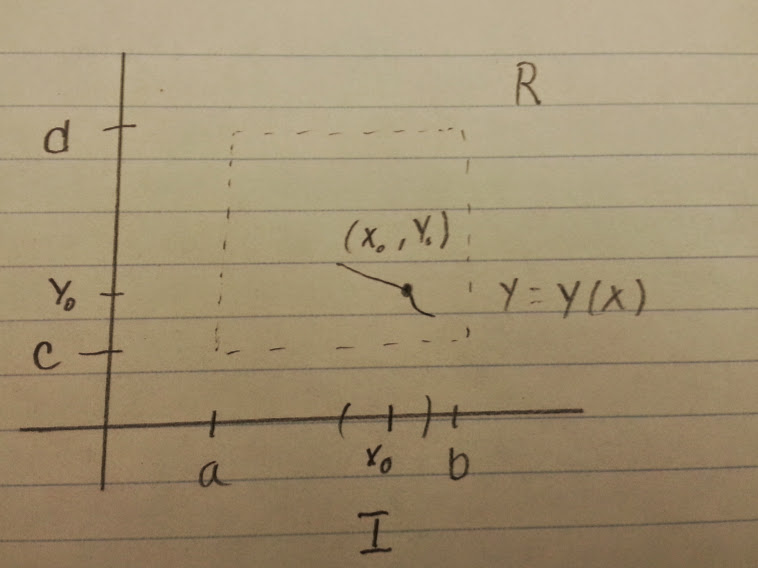
\includegraphics[scale=.45]{pic1}
  
  \begin{tikzpicture}[scale=.6]
  
     
    %\draw[step=1cm, teal, very thin] (0,0) grid (10,10); % Grid lines
  
    \draw[thick, ->] (-1,0) -- (10,0) % + x axis line
    	node[anchor=north west] { \( x \) }; % x axis lable 
  
    \draw[thick,->] (0,-1) -- (0,10) % + y axis line 
    	node[anchor=south east] { \( y \) }; % y axis lable

    \draw[very thick, red]
    (4,5)  to [out=60, in=180] (6,2.99) to [out=0, in=128] (8,2.3); 

    \draw[fill] (6,3) circle [radius=2pt] % dot in top right corner
    	node[above right]  { \( (x_0, y_0) \)}; % lable (10,10) 

    \draw[thick,  dashed] 
    (2,2) -- (2,9) -- (9,9) node[above right] { \( R \)} --
    (9,2) -- (2,2);
  
    \draw[thick]
    (-.5,9) node[left] { \( d \)} -- (.5,9);

    \draw[thick]
    (-.5,3) node[left] { \( y_0 \)} -- (.5,3);

    \draw[thick]
    (-.5,2) node[left] { \( c \)} -- (.5,2);

    \draw[thick]
    (2,-.5) node[below] { \( a \)} -- (2,.5);
   
    \draw[thick]
    (9,-.5) node[below] { \( b \)} -- (9,.5);

    \draw[thick]
    (6,-.5) node[below] { \( x_0 \)} -- (6,.5);

    \node [red, below] at (11,3) { \( y=y(x) \)};
    
  \end{tikzpicture}
  \\[5mm]

  \[ R = (a, b)x(c, d)\]
  \[ = {(x, y) \in R^2 | a < x < b \text{ \& }  c < y < d } \]
  The \( \exists \text{! thrm} \) is a "local" result, local \\
  to \(x_0\), move precisely, it just sups that there is a unique soln in I \\
  not necessarily outside of I. \\

  \subsection*{Ex(p.29) \# 27}
  
  \[ y' = s \sqrt{y} \text{ \& } y(0) = 0\]
  consider 
  \[ y(x) = \left\{
  \begin{array}{l l}
	0 & x\leq c \\
	(x-c)^2 &  x \geq c
  \end{array}\right. \]
  which is ctn on \( \mathbb{R} \)  \\
  notice that both parts  \\
  y(x) satisfy the initial value problem if \\
  \( c \geq 0\) Note: 

  % pic
  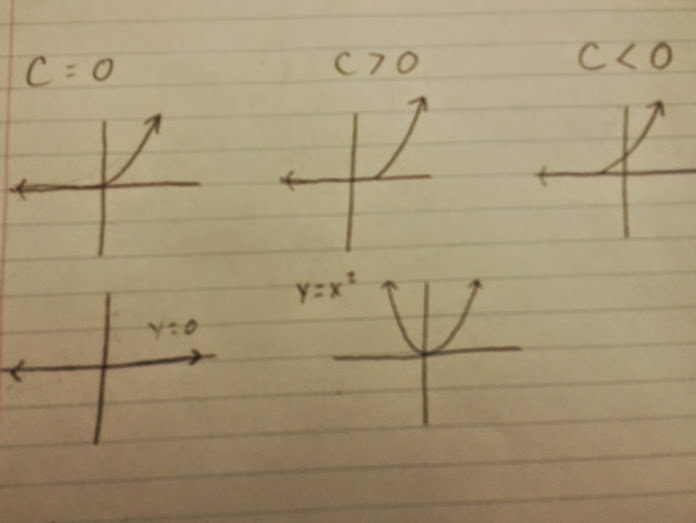
\includegraphics[scale=.45]{pic2}

  Notice that
  \[ f(x, y) = 2\sqrt{y} \text{ \& } f_y(x, y) = \frac{1}{ \sqrt{y}}\]
  which is cts on \( R = \{ (x, y) \in R^2 |  y > 0\}\)

  % pic 
  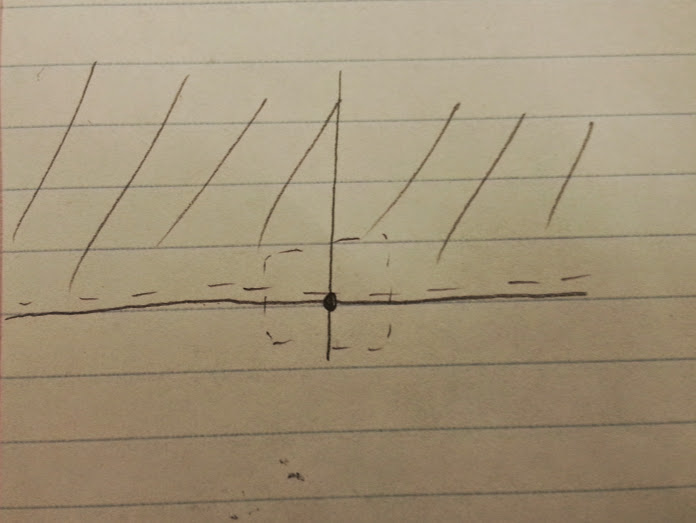
\includegraphics[scale=.45]{pic3}

  notice that (0, 0) is not in R, not \\
  "interior" to R. \( \therefore \exists \text{! thrm}\) does not apply
  \\
  Notice that if \( y = f(x) \) is a soln to \\
  an ODE on a interval I  \\
  then so is \( y = f(x-c)\) a soln to  \\
  the ODE on \( I - c =\{ x \in R | x + c \in I\}\).  \\
  % }}} 

  % Date: 02.03.2015 ------------------- {{{
  \newpage 
\marginpar{Date: 02.03.15.}
%\section{Date: 02.03.2015}
  \subsection*{ ex p.28 }
  15. \( y' = \sqrt{x-y} \text{ ,  } y(2) = 2 \),  no \\
  16. \( y' = \sqrt{x-y} \text{ ,  } y(2) = 1 \),  yes \\
  here \( f(x, y) = \sqrt{x-y}\) , which has \\
  cts iff  \( x-y \geq 0 \iff x \geq y\) \\ 
  \( f_y(x, y) = - \frac{1}{2\sqrt{x-y}}\),  which is cts \\
  on \( \{ (x,y) \in \mathbb{R}^2 \text{ | } y<x \}\). \\
  \subsection*{ Notes \\ } 
  Def A first order linear ODE \\
  has the form
  \[ \text{ (1) } y' + p(x)y = q(x)\] 
  where p \& q are cts on some interval \( \mathcal{I}\). \\
  Notice that if \( q(x) = 0\) then (1) is \\	
  separable. \\	  
  Key observation: the left side of \\
  (1) resembols the product rule. \\
  this motivates a question: Is there \\
  a cst I(x), say on the interval \( \mathcal{I}\),  \\
  st  \\
  (1') \( y'I(x) + yp(x)I(x) = q(x)I(x)\) ,  \\
  where the left side of (1') is the dirivative  \\
  of a product? \\

  if there is such an I(x)  \\
  then  \\
  (2) \( I'(x) = p(x)I(x)\). \\
  put \( v = I(x)\), then (2) becomes  \\
  \[ v' = p(x)v\]
  which is separable. thus \nonumber\\
  \[ \frac{v'}{v} = p(x) \implies\]
  \[ \int \frac{1}{v}dv = \int p(x)dx \implies\]
  \[ \ln|v| = \int p(x)dx + C \implies \]
  \[ |v| = e^{\int p(x)dx + C} = Ke^{\int p(x)dx}\]
  where \( k > 0 \therefore\)
  \[ v = Ke^{\int p(x)dx} \text{ , } K \neq  0\]
  Def. the intergrating factor of 
  \[ y' + p(x)y = q(x) is \]
  \[ I(x) = e^{\int p(x) dx }\]
  Finally, from (1') 
  \[ (yI(x))' = q(x)I(x) \implies \]
  \[ yI(x) = \int q(x)I(x)dx \implies\] 
  \[ \boxed{ y = \frac{1}{I(x)} \int q(x)I(x)dx}\]
  % }}}
 
  % Date: 02.04.2015 -------------------------- {{{
  \newpage
\marginpar{Date: 02.04.15.}
%\section{Date: 02.04.2015}

\subsection*{Single Tanking Problem}
 \( c_i\) = concentration coming into the tank (constant) \\
 \( r_i\) = rate of flow into the tank (constant) \\
 \( c_0(t)\) = concentration coming out of the tank \\
 \( r_0\) = rate of flow out of the tank (constant) \\
 \( x(t) \) = amount of salute in tank at time t \\
 \( V(t)\) volume of tank at time \( t\) \\[5mm] 
 Units: \\
 Concentration = \( \frac{ \text{ amount of solute }}{ \text{ unit
 valume	 }}\) \\ 
 Rate = \( \frac{ \text{ valume }}{ \text{ unit time }}\) \\	 
 amount = (concentration)(rate)(time) \\[5mm]
 Notice that the rate of change fo the volume is constant and  \\
 is \( m = r_i - r_0\); where, \( V(t) = (r_i - r_0)t + V_0 = mt +
 V_0\), where \( V_0 = V(0)\) \\
 For a small \( \Delta t\)\nonumber\\
 \( x(t + \Delta t) = x(t) + \text{ amount in = amount out over time }
 \Delta t\) \\[5mm]
 amount in over \( \Delta t = c_i r_i \Delta t\); \\
 amount out over \( \Delta t \approx c_0(t) r_0 \Delta t\). \\
 thus,  \\
 \[ \Delta x = x(t + \Delta t) - x(t) \approx (c_i r_i - c_0(t)r_0) \Delta
 t \implies \]

 \[ \frac{\Delta x}{\Delta t} \approx c_i r_i - c_0 (t) r_0\]
 this suggest that  \\
 \[ \frac{dy}{dx} = c_i r_i - c_0 (t) r_0\]
 Now\nonumber\\
 \[ c_0(t) = \frac{x(t)}{V(t)} \implies \]
 \[ \frac{dx}{dt} = c_ir_i = \frac{x(t)}{V(t)}r_0\]
 which is a 1st order linear ODE. \\
 more consiely, put \( x' = \frac{dx}{dt}\) and \\
 \( x= x(t) \), then  \\
 \[ \boxed{x' + \frac{r_0}{V(t)}x = c_ir_i}\]
 Recall that \( V(t) = mt + v_0 \text{ , } m = r_i - r_0\); so,  \\
 \[ x' + \frac{r_0}{mt + v_0} x = c_ir_i\] 
 Here  \\
 \[ p(t) = \frac{r_0}{mt + V_0} \implies\]
 \[ \int p(x) dx = \frac{r_0}{m} ln (mt + V_0) + C\] 
 where in context, \( V(t) > 0\). Choose, of ease, \\ 
 \( C = 0\), then \\
 \[ I(t) = e^{\int p(t)dt} = (mt + V_0)^{r_0/m}\]
 So,  \\
 \[ x'(mt + V_0)^{r_0/m} + r_0(mt + V_0)^{r_0/m -m } = c_ir_i(mt +
 V_0)^{r_0/m} \implies \]
 \[ (x(mt + V_0)^{r_0/m})' = c_ir_i+(mt + V_0)^{r_0/m} \implies\]
 \[ x(mt+V_0)^{r_0/m} = c_ir_i \int (mt +V_0)^{r_0/m}dt\]
 If \( r_0/ m = -1 \) then \( r_0 = -m = -r_i + r_0\) \\
 \( \implies r_i = 0 \), which is not of intrest in \\ 
 context ("mixing").  Thus, if \( r_0/m \neq -1\) \\
 then 
 \[ \int (mt + V_0 )^{r_0/m}dt = \frac{1}{m}(mt + V_0)^{r_0/m +
 1}\frac{m}{r_0 + m} + C\]
 \[ = \frac{1}{r_i}(mt + V_0)^{r_i/m} + C\]
 \[ \therefore\]
 \[ x(mt + v_0)^{r_0/m} = c_i(mt + V_0)^{r_i/m } + C\]
 at \( t = 0\)
 \[ x_0V_0^{r_0/m} = c_iV_0^{r_i/m} + C \implies\]
 \[ C = c_iV_0^{r_i/m} - x_0V_0^{r_0/m}\]
 \[ = V_0^{r_0/m}(c_iV_0 - x_0)\]
 thus, 
 \[ x(mt + V_0)^{r_0/m} = c_i(mt+V_0)^{r_0/m} + V_0^{r_0/m}(c_iV_0 -x_0\]
 \[ \implies x = c_i(mt + V_0) + (c_iV_0 - x_0)
 (\frac{V_0}{mt+V_0})^{r_0/m}\]

 \begin{empheq}[box=\fbox]{align}
	x = c_iV + (c_iV_0 - x_0)
	\bigg(\frac{V_0}{V}\bigg)^{r_0/(ri-r_0)} \nonumber \\
	\text{ where } x = x(t) \text{ \& } V = (r_i-r_0) t + V_0
	\nonumber 
 \end{empheq} 

 %\[ \boxed{x = c_iV + (c_iV_0 - x_0) (\frac{V_0}{V})^{r_0/(ri-r_0)} \\
 %\text{ where } x = x(t) \text{ \& } V = (r_i-r_0) t + V_0}\]

 % }}}  

%\section{Date: 02.05.2015 } 

 % Date: 02.09.2015 ------------------------ {{{
 \newpage 
\marginpar{Date: 02.09.15.}
\section{Date: 02.09.2015}
  1.6 Substitutions in ODEs \\
  Consider a slope field  \\
  \[ \text{ (1) } \frac{dy}{dx} = f(y, x)\]
  i.e., a 1st order normal ODE. If
  \[ \alpha (x, y)\]
  appers in (1), then we are compelled  \\
  to make the substitution  \\
  \[ v = \alpha (x, y)\]
  ("alpha" for auxillary variable) \\
  By the calc III chain rule\nonumber\\
  \[ \frac{dv}{dx} = \frac{\partial\alpha}{\partial x} \frac{dx}{dx} + \frac{\partial
  \alpha}{\partial y} \frac{dy}{dx}\]
  
  \[ = \alpha_x + \alpha y \frac{dy}{dx}\]
  
  If \( v = \alpha (x, y) can be soved \) \\
  for y in terms of x and v, say  \\
  \[ y = \beta(x, v) \] \\
  then from (1), we have that  \\
  \[ \frac{dv}{dx} = \alpha_x + \alpha_y \frac{dy}{dx} = \alpha +
  \alpha_y f(x, y) \]
  where, 
  \[ \boxed{ \frac{dv}{dx} = \alpha_x + \alpha f(x, \beta(x, v))}\]

  which is a new ODE with dependent variable v
  and independent variable x. 
  \subsection{ex}
  \[ \frac{dy}{dx} = f(x, y , ax+by+c\]
  put 
  \[ v + d(x, y) = ax + by + c\]
  then 
  \[ \frac{dv}{dx} = a + b \frac{dy}{dx}\]
  thus, 
  \[ \frac{dv}{dx} = a + b \frac{dy}{dx} = a + b f(x, y, ax + by +c)\]
  \[ \implies \boxed{\frac{dv}{dx} = a + b f(x, (v-ax-c)/b, v)}\]
  where 
  \[ y = \beta (x, v) = \frac{v-ax-c}{b} \text{ , } b \neq 0\]

  \subsection{p.74 16}
  \[ y' = \sqrt{x+y+1}\]
  \[ v = x + y + 1 \implies y = v - x - 1 \text{ \& } \]
  \[ \frac{dv}{dx} = 1 + \frac{dy}{dx} \implies \]
  \[ \frac{dv}{dx} = \sqrt{v} + 1 \text{ (separable) }\]

  Def. A first order normal homogenous 
  ODE has the form 
  \[ \frac{dy}{dx} = f(y/x)\]

  \subsection{Ex}
  \[ y' = \frac{xy}{x^2 + y^2}\]
  In general, put 
  \[ v = \alpha (x, y) = y/x \text{ (slope) }\]
  so, \( y = xv\) implies that 
  \[ f(v) = f(y/x) = \frac{dy}{dx} = v + x \frac{dv}{dx} \implies \]
  \[ x \frac{dv}{dx} = f(v) - v \text{ (separable) }\]
  \[ \frac{1}{f(v) -v} \frac{dv}{dx} = \frac{1}{x} \implies \]
  \[ \int \frac{1}{f(v) -v} dv = \ln |x| + c\]

  \subsection{Ex (Revisited)}

  \[ y' = \frac{xy}{x^2 + y^2} = \frac{y/x}{1 + (y/x)^2} , v = y/x
  \implies \]
  \[ \int \frac{1}{\frac{v}{1 + v^2} -v}dv = \ln |x| + c \implies \]
  \[ - \int \frac{1 + v^2}{v^3}dv = \ln |x| + c \implies \dots \]
  % }}}

  % Date: 02.10.15 ------------------- {{{
  \newpage 
\marginpar{Date: 02.10.15}
\section{Date: 02.10.2015}
  Thrm. If \( p(x, y) = \sum a_{i_1 i_2} x^{i_1} y^{i_2} \) and \\
  \( Q(x, y) = \sum a_{j_1 j_2} x^{j_1} y^{j_2} \) are polynomials \\
  over \( \mathbb{R} \), then if there is a \( k \in \mathbb{Z}^+ \) st
  for all \( i_1, i_2, j_1, j_2,  \)
  \[ i_1 + i_2 = d = j_1 + j_2 \]
  then \( p(x, y)y'=Q(x, y)  \) is a 1st order linear \\
  homogenous ODE.\\
  Proof. notice that 
  \[ y' \sum a_{i_1 i_2} x^{i_1} y^{i_2} = 
  \sum a_{j_1 j_2} x^{j_1} y^{j_2} \implies \]

  \[ \frac{1}{x^d} y' \sum a_{i_1 i_2} x^{i_1} y^{i_2} = 
  \frac{1}{x^d} \sum a_{j_1 j_2} x^{j_1} y^{j_2} \implies \]

  \[ y' \sum a_{i_1 i_2} \frac{y^{i_2}}{x^{d-i_1}} =
   \sum b_{j_1 j_2} \frac{y^{j_2}}{x^{d-j_1}} \implies\]
   
   \[ y' \sum a_{i_1 i_2} (\frac{y}{x})^{i_2} =
   \sum b_{j_1 j_2} (\frac{y}{x})^{j_2}  \implies\]
   
   \[ y' =  \frac{\sum a_{i_1 i_2} (\frac{y}{x})^{i_2}}{\sum b_{j_1 j_2} (\frac{y}{x})^{j_2} }\]
   which is hom. endproof

   Def. (i) deg \( a_{i_1, i_2 ...i_n} x_1^{i_1}, x_2^{i_2}, \dots
   x_n^{i_n} = \sum_{k=1}^{n} i_{k i}\)

   (ii) deg \( ((p(x_i)) \)
   
   where \( p(x_1, x_2, \dots , x_n = \sum a_{i_1 i_2 \dots i_n}
   x_1^{i_1} x_2^{i_2} \dots x_n^{i_n} \)

   \subsection{ex p.74 2} 

   \[ 2xyy' = x^2 +2y^2 \implies  \]
   \[ y' = (\frac{1}{2} \frac{1}{y/x} + 2(y/x)) \text{ , } v = y/x
   \implies \]
   \[ y = vx \implies y' = v + xv' \text{ \& } xv' +v = \frac{1}{2v} +v
   \implies \]
   \[ v' = \frac{1}{2xv} \text{ (separable) } \implies  \]
   \[ vv' = \frac{1}{2x} \implies \]
   \[ \int v dv = \frac{1}{2} \int \frac{1}{x} dx = \frac{1}{2} \ln |x|
   \implies \]
   \[ \frac{v^2}{2} = \frac{1}{2} \ln |x| + c \implies  \]
   \[ v^2 = \ln |x| + c \implies  \]
   \[ v = +- \sqrt{ \ln |x| + c} \implies \]
   \[ \frac{y}{x} +- \sqrt{\ln |x| + c} \implies  \]
   \[ y = +-x \sqrt{\ln |x| + c} \]
   Def. A first order (normal) \\
   berelli ODE has the 
   \[ y' +yp(x) = y^nq(x) \]

   side note(good book) Asmov PDE 
\section{Date: 02.11.2015}
  Recall: Bernulli ODE
  \[ y' + yp(x) = y^n q(x) \]
  put \( v = y^m \) then
  \[ \frac{dv}{dx} = my^{m-1} \frac{dy}{dx} \implies \]
  \[ my^{m-1} \frac{dy}{dx} + my^m p(x) = my^{m+n-1}  q(x) \implies \]
  % needs perp sign
  \[ \frac{dv}{dx} vmp(x) = my^{m+n-1}  q(x)\]
  want: \( m+n-1=0 \). this requires \\
  that \( m = 1-n \). \( \therefore v=y^{1-n}\) reduses \\
  a bernoulli ODE to a 1st order linear ODE. \\

  \subsection{p.74 25}
  \[ y^2(xy'+y)(1+x^4)^{1/2} = x \]
  \[ \implies (xy^2y' + y^3) \sqrt{1+4x} = x\]
  \[ \implies xy^2y' \sqrt{1+x^4} + y^3 \sqrt{1+x^4} = x \]
  \[ \implies y' \sqrt{1+x^4} + y \frac{ \sqrt{1+x^4}}{x} = y^{-2} \]
  \[ \implies y' +y \frac{1}{x} = y^{-2} \frac{1}{ \sqrt{1+x^4}} \]
  put \( v = y^3 \) then 
  \[ \frac{dv}{dx} = 3y^2 \frac{dy}{dx} \implies \]
  \[ 3y^2y' + \frac{3y^3}{x} = \frac{3}{ \sqrt{1+x^4}} \implies \]
  \[ v' + \frac{3v}{x} = \frac{3}{ \sqrt{1+x^4}} \text{ (linear) } \]
  Here \( p(x) = 3/x \); so\nonumber\\
  \[ I(x) = e^{\int p(x)dx} = e^{3\ln |x|} = x^3 \]
  Thus, 
  \[ v'x^3 ' + v3x^2 = \frac{3x^3}{ \sqrt{1+ x^4}} \implies \]
  \[ (vx^3)' = \frac{3x^3}{ \sqrt{1+x^4}} \implies \]
  \[ vx^3 = 3 \int \frac{x^3}{ \sqrt{1 + x^4}}dx = 
  \frac{3}{4} \int w^{-1/2} dw\]
  \[ \frac{3}{4} \frac{2}{1}w^{1/2} + c\]
  \[ \frac{3}{2} ( \sqrt{1+x^4} + c \]
  \[ w = 1+x^4  \]
  \[ w' = rx^3 \]
 % need stuff

 \[ y^3 = \frac{3}{2} ( \frac{ \sqrt{1+x^4} + c}{x^3}) \implies  \]
 \[ y =  (\frac{3}{2} ( \frac{ \sqrt{1+x^4} + c}{x^3}))^{1/3}\] 

 % }}}

 Exam 1 
 1. Given an ODE and a soln to it, verify it is a soln, then find a
 particular soln givin an initial cond.

 2. Given a description of an ODE, write down the ODE. 

 3. Dropping ball from some h, find , ground time and speed.

 4. high jump on earth given, find high jump on jupiter. 

 5. (a) solve ODEs 
 
(b) 

one is separable and the other is linear or bornulli

6. Torricelli problem. 


\chapter{Second Test}

% vim:tw=72 sw=2 ft=tex
%         File: test2.tex
% Date Created: 2015 Feb 17
%  Last Change: 2015 May 16
%     Compiler: pdflatex
%       Author: joshua
\documentclass[10pt,a4paper]{article}
\usepackage{amsmath, amssymb}
\usepackage{amsthm}
\usepackage[utf8]{inputenc}
\usepackage[T1]{fontenc}
\usepackage[english]{babel}
\usepackage{graphicx}
\usepackage{mathrsfs} % gives me a font I need
\usepackage[document]{ragged2e} % flush everything left dont wory about
% the error

\DeclareMathOperator\arctanh{arctanh}
\DeclareMathOperator\sech{sech}


\newtheorem*{theorem}{Theorem}
\newtheorem*{corollary}{Corollary}

\theoremstyle{definition}
\newtheorem*{definition}{Definition}
\newtheorem*{example}{Example}

\everymath{\displaystyle}


\graphicspath{ {./images/} }

\begin{document}
%\title{Notes for Second Test}
%\author{Joshua Bailey}
%\maketitle
%\newpage

% Date 02.17.15. --------------------------  {{{
\marginpar{Date: 02.17.15.}
\begin{example}
  \[ (2x \sin y \cos y ) y' = 4x^2 + \sin^2y \]
  \[ v = \sin y \implies\]
  \[ \frac{dv}{dx} = \cos y \frac{dy}{dx} \]

  Thus, 
  \[ 2xvv' = 4x^2 + v^2 \text{ (hom),  } w = v/x \]
\end{example}

\section{population models}

  Recall that the most basic population model, \\ 
  assuming constant birth and death rates, is 

  \[ P' = kP \text{ (separable)  } \]

  Now, we give birth rates and death rates the \\
  following units: 

  \[ \beta(t) = \text{ birth rate } \frac{ \text{ \# of births at t }}{
  \text{ (unit of population at t)(unit of time) }} \]

  \[ \delta(t) = \text{ death rate } \frac{ \text{ \# of death at t }}{
  \text{ (unit of population at t)(unit of time) }} \]

  with this, for some small \( \Delta t \), 

  \[ P(t + \Delta t) \approx P(t) + \text{ ( \# birth rate at t - \# death rate at t) } \Delta t \implies   \]
  \[ = P(t) + \beta (t) P(t) \Delta t - \delta (t) P(t) \Delta t \]
  \[ \implies \frac{ \Delta P}{ \Delta t} =  \frac{P(t + \Delta t) -P(t)}{ \Delta
  t}  \approx ( \beta(t) - \delta(t) ) P(t)  \]

  using a diff model, the above suggest that 

  \[ \boxed{ P' = (\beta - \delta ) P} \]

  This is called the general population \\[5mm]

  Now, consider population with constant 
  death rate, say \( \delta_0 \), and with a birth 
  rate given by 

  \[ \beta = \beta_1 - \beta_0P \]

  In context, \( \beta_0 \text{ , } \beta_1 > 0 \) by (1),

  \begin{align*}
    P' &= ( \beta_1 - \beta_0 P -\delta_0 ) P \\
    &= ( \beta_1 - \delta_0 ) P - \beta_0 P^2 \\
    &= \beta_0 P  \left( \frac{ \beta_1-\delta_0}{\beta_0} -P \right)  
  \end{align*}

  which has form 
  \[ P' =  kP(M-P) \]
  \( k = \beta_0 > 0 \) and \( M = (\beta_1 -\delta_0)/ \beta_0  \) we
  see that in context, M>0 here (2) 
  is separable; as 
  \[ \frac{P'}{P(M-P)} =k \implies  \]
  \[ \int \frac{1}{P(M-P)}dP = kt + C \]
  Note that

  \[ \frac{1}{P(M-P)} = \frac{1}{M} \bigg( \frac{1}{M-P} +
  \frac{1}{P}\bigg) \]

  Thus, 

  \[ \frac{1}{M} (- \ln | M-P| + \ln|P|) = kt + C \implies  \]
  \[ \ln \bigg| \frac{P}{M-P} \bigg| = Mkt + C \]

  Now, \( P_0 = P(0) \) yields 

  \[ C = \ln \bigg| \frac{P_0}{M - P_0}\bigg|  \]
  Thus,

  \[ \ln \Big| \frac{P}{M-P} \bigg| = \ln \bigg| \frac{P_0}{M - P_0}\Big| + Mkt\]

  Hence, if \( P > M \) or \( P_0 > M \) then  

  \[  \frac{P}{M-P} = \frac{P_0}{M - P_0} e^{Mkt} \implies \frac{M}{P}
  -1 =  \frac{M - P_0}{P_0} e^{-Mkt}\]
  \[ \implies  \frac{M}{P} = \frac{P_0 + (M-P_0)e^{-Mkt}}{P_0} \]
  \[ \boxed{P(t) = \frac{MP_0}{P_0 + (M-P_0)e^{-Mkt}} } \]
  Notice that
  \[ \lim_{t \to \infty} P(t) = \frac{MP_0}{P_0} = M \]
  If \( P<M \), so that \( P_0 < M \), then
  \[ P' = kP(M-P) > 0 \]
  so, P is increasing to M \\[5mm]
  On the other hand, if \( P > M \), so \\
  that \( P_0>M \), then 
  \[ P' = kP(M-P) <0 \]
  so, P is decresing to M \\
  Since \( P(t) \to M \) in \\
  either case, in context,  \\
  \( M>0 \), \(  ( M = 0 \text{ \& } P>M \implies extinction) \). \\
  % }}}  

  % Date: 02.19.15. ----------------------------- {{{
  \newpage  
  \marginpar{Date: 02.19.15.}
  Recall: logistics population model 
  \[ P(t) = \frac{MP_0}{P_0 + (M - P)e^{-Mkt}} \]

  \begin{example}
    Page 88 Problem \# 22 \\
    \(M=100 \times 10^3 \) total population At \( t=0 \), half the
    population have heard a rumor, roughly the rumors increases by 1000
    people after 1 day 

    \[ P_0 = 50 \times 10^3 \text{ \&   } P(1) = 51 \times 10^3 \]

    we can solve for k

    \[ 51 \times 10^3 = \frac{(100 \times 10^3) (50 \times 10^3)}{ 50
    \times 10^3 + (100 \times 10^3 - 50 \times 10^3) e^{-Mk}} \]
    \[ \implies 51 = \frac{5000}{50 +50e^{-Mk}} = \frac{100}{1+e^{-Mk}} \]
    \[ \implies \frac{51}{100} = \frac{1}{1+e^{-Mk}} \implies  \]
    \[  1+ e^{-Mk} = \frac{100}{51} \implies  e^{-Mk} = \frac{100}{51} -1
    \implies \]
    \[ -Mk = \ln \bigg( \frac{100}{51} -1 \bigg) \]
    \[ \implies k= - \frac{\ln ( \frac{100}{51} - 1)}{10 \times 10^3} > 0 \]

    Therefore we can now solve \( P(t) = 80 \times 10^3 \) \\
    for t. \\

  \end{example}

\section{Doomsday/Extinction Model:} 

  Here we assume that 
  \[ \beta = kP, \text{  } k>0 \]
  \[ \text{ \& } \delta  = \delta_0 \]

  Thus, the gen pop ODE, \( P' = (\beta -\delta )P \), becomes 

  \begin{equation}
    \tag{1}
    \label{Model1}
    P' = (kP-\delta_0)P = kP(P-\delta/k )
  \end{equation}

  put \( M = \delta / k > 0 \),
  \eqref{Model1} becomes

  \begin{equation}
    \tag{2}
    \label{Model2}
    P' = kP(P-M)
  \end{equation}

  constant \eqref{Model2} with the logistics \\
  ODE: \( P' =kP(M-P) \) we 
  can solve \eqref{Model2}; it is separable. Thus,
  \[ \frac{P'}{P(P-M)}= k \implies  \]
  \[ \int \frac{1}{P(P-M)}dP = kt + C \]

  Note:

  \[ \frac{1}{P(P-M)} = \frac{1}{M}( \frac{1}{P-M}- \frac{1}{P}) \]

  Therefore 

  \[ \frac{1}{M}( \ln|P-M| - \ln P ) = kt + C \]
  \[ \implies \ln  \bigg| \frac{P-M}{P}\bigg| = Mk + C \]
  \[ \implies \frac{|P-M|}{P} = e^{Mkt+C} \]

  If \( P_0 = P(0) \) then 

  \[ C = \ln \bigg|\frac{P_0-M}{P_0}\bigg| \]

  so,

  \[ \frac{P-M}{P} = \frac{P_0-M}{P_0}e^{Mkt} \]

  Now, in any case 

  \[ \frac{P-M}{P} = \frac{P_0 - M}{P_0}e^{Mkt} \implies \]
  \[ 1 - \frac{M}{P} = \frac{P_0-M}{P_0}e^{Mkt} \implies  \]
  \[ \frac{M}{P} = \frac{P_0- (P_0 -M) e^{Mkt} }{P_0} \implies  \]
  \[ \boxed{P = \frac{MP_0}{P_0 + (M-P_0)e^{Mkt}} } \]

  contrast with logistic ODE soln: 

  \[ P = \frac{P_0M}{P_0 + (M-P_0)e^{-Mkt}} \]

  % }}}

  % Date: 02.23.15. ------------------------------  {{{
  \newpage
  \marginpar{Date: 02.23.15.}
\section*{With explosion/extinction modol}

  Notice that 

  \[ P>M \implies P'>0 \implies P \text{ is increasing; } \]
  \[ P>M \implies P'<0 \implies P \text{ is decreasing; } \]

  Now, if \( P>0 \), then P has a vertical 
  asymptote at \( t_0 \) such that. 

  \[ P_0 + (M-P_0)e^{Mkt_0} = 0 \implies \]
  \[ e^{Mkt_0} = \frac{P_0}{P_0 - M}>0 \implies \]
  \[ Mkt_0 = \ln \frac{P_0}{P_0-M} \]
  \[ \boxed{t_0 = \frac{1}{Mk} \ln \bigg( \frac{P_0}{P_0-M} \bigg)} \]

  which is the time of "doomsday," i.e., the explosion of the population 

  \[ \lim_{t \to t_0^-} P(t) = \infty \]

  On the other hand, if \( P<M \), then \( M-P_0>0; \) the

  \[ \lim_{t \to \infty} P(t) = 0 \]
  j
  This is to say, over time, extinction occurs. 

  % }}}

  % Date: 02.24.15. ----------------------------- {{{
  \newpage 

  \marginpar{Date: 02.24.15}
\section*{equilibuim solns and stability}

  Def. An autonomous ODE has the form 

  \begin{equation}
    \tag{1}
    \label{autonomous ODE}
    \frac{dx}{dt} = f(x) 
  \end{equation}

  Notice that the slope field in \eqref{autonomous ODE} is "independent"
  of t.

\section*{ Newtons law of cooling} 

  \[ T' = k(A-T) \text{ , } k>0 \]

  Recall:

  \[ \int \frac{1}{A-T}dt = \int kdt = kt + C \implies \]
  \[ -\ln |A-T| = kt +C \implies  \]
  \[ |A-T| = e^{-kt-C} \]

  where \( T_0 = T(0) \implies  \)

  \[ -C = \ln |A-T_0|  \] 

  thus, 

  \[ |A-T| = |A-T_0|e^{-kt} \implies \]
  \[ A-T = (A-T_0)e^{-kt} \implies \]
  \[ \boxed{T(t) = A + (T_0-A)e^{-kt} } \]

  Notice that 

  \[ \lim_{t \to \infty} = A \]

  Also, notice that \( T(t) \equiv A \),  i.e, \( T(t) = A \) for all t,
  in a soln to the autonomous ODE \( T' = k(A-T) \). this is  an example
  of an "equilibruim soln" \\[5mm] 

  \begin{definition}
   \( x(t) \equiv  C \in \mathbb{R} \) is an equilibrium soln to \( x' =
   f(x) \text{ iff } x(t) \equiv C \) is a soln to \( x' = f(x) \)
  \end{definition}

  \begin{definition}
   \( x = C \in \mathbb{R}  \) is a critical point of \( x' = f(x) \) iff \( f(c) = 0 \)
  \end{definition}

  Notice that we say that "x is a critical point" iff \( 0 = f(C) =
  \frac{dx}{dt} \), which is similar to use in calc I of  "critical pt." \\[5mm]

  Prop. \( x=C \) is a critixcal pt \\
  of \( x'=f(x) \iff x(t) \equiv  C \) \\
  is an equilibrium soln to \( x' = f(x) \) \\
  proof. easy. \\[5mm] 
  Def. \( C \in \mathbb{R} \) is a stable critical \\
  point of \( x' = f(x) \) iff C is a \\
  critical pt of \( x' = f(x)  \) and \\
  \[ \forall \epsilon >0 \text{  } \exists \text{  } \delta >0 \forall \]
  \[ |x_0 -C| < \delta  \implies |x(t) -C| < \epsilon  \]

\section*{Ex (Logistics Modle)}
  \[ P' = kP(M-P) \implies \]
  \[ P(t) = \frac{MP_0}{p_0 + (M - P) e^{-Mkt} } \implies  \]
  \[ \lim_{t \to \infty}P(t) = M \]

  Ex(Standard pop Model) 

  \[ P' = kP \implies P(t) = P_0 e^{kt}  \]
  Here \( P=0 \) is a critical pt; however, \\
  \( P=0  \) is not stable. 
  Notice that \( P' = kP(M-P)  \) has two \\
  critical pts, namely, \( P = 0 \) and \( P =M \). \\
  Here \( P(t) = M \) is stable, whereas, \( P(t) \equiv 0 \) is not \\
  stable.  \\[5mm]  
\section*{Ex(explosion/ extinction model)}
  \[ P' = kP(P-M) \text{ , } k, M>0\]
  \[ \implies P(t) = \frac{MP_0}{P_0 + (M-P_0)e^{Mkt}} \]
  Both \( P=0 \) and \( P=M  \) are \\
  critical pts. however, if \( P_0 > M \) \\
  then ? a stable, whereas \\
  if \( P_0 <M  \)then only \( P=0 \) \\
  is stable.
  \[ |x_0 - C| < \delta  \implies  \]
  \[ (x(t) -C) < \epsilon  \]

  % }}} 

  % Date: 02.25.15. ------------------- {{{
  \newpage 
  \marginpar{Date: 02.25.15.}
\section{Logistics Population Model with  Harvesting}

  Recall the Logistics Pop Model: 

  \[ P' = kP(M-P) \text{, }k \text{, } M>0  \]

  We now consider

  \[ P' = kP(M-P)-h \]

  where h is a constant, think: \( h>0 \implies \) harvesting; \\

  \[ h<0 \implies \text{ stocking } \]

  Notice that 
  \begin{align*}
  P' &= -kP^2 + kMP -h \\
   &= -k(P^2 -MP + h/k) \\
   &= -k(P-N)(P-H) 
  \end{align*}

  where

  \[ \text{ H,N  } = \frac{M \pm \sqrt{M^2 -4h/k}}{2} \]

  Here H and N are distinct reals if and only if \( M^2 -4h/k > 0 \iff
   M^2 >4h/k \iff h<kM^2/4 \). so, if \( h>0 \) and H, N are distinct
   and real, then 

  \[ 0 < h< \frac{kM^2}{4} \]

  Say, H<N. Notice that 

  \[ h>0 \implies \]
  \[ \sqrt{M^2 -4h/k} <  \sqrt{m^2} \implies  \]
  \[ M- \sqrt{M^2 - 4h/k} > 0 \]
  \[ \therefore 0<H \text{ ; where,  } 0< H < N  \]
  Now, "separating,"  yields that 
  \[ \frac{P'}{(P-H)(P-N)} = -k \implies \]
  \[ \int \frac{1}{(P-H)(P-N)}dP = -kt + C  \]
  Notice that 
  \[ \frac{1}{(P-H)(P-N)}= \bigg(\frac{1}{P-N} - \frac{1}{P-H}\bigg) \frac{1}{N-H} \]
  Thus, 
  \[ \ln \bigg| \frac{P-N}{P-H}\bigg| = -(N-H)kt + C \]
  If \( P_0 = P(0)  \) then
  \[  C = \ln \bigg| \frac{P_0-N}{P_0-H}\bigg| \]
  Hence \(  \big| \frac{P-N}{P-H}\big| = e^c e^{-(N-H)kt} = \big| \frac{P_0-N}{P_0-H}\big| e^{-(N-H)kt}\)
  Now, in any case, 
  \[ \frac{P-N}{P-H} =  \frac{P_0-N}{P_0-H} e^{-(N-H)kt}\]
  \[ \lim_{t \to \infty} \frac{P-N}{P-H} = \lim_{t \to \infty} \frac{P_0-N}{P_0-H} e^{-(N-H)kt}	 \]
  \[ \therefore \lim_{t \to \infty}(P-N) =0 \text{ or } \lim_{t \to
  \infty} (P-H) = \pm  \infty  \]
  Q: Is \( N<M \)? \\
  Q; \( P(t) =  \)?
  % }}}

  % Date: 02.26.15 ------------------ {{{
  \newpage
  \marginpar{Date: 02.26.15 }
  Recall: 
  \[ \frac{P-N}{P-H} =  \frac{P_0-N}{P_0-H} e^{-(N-H)kt} \implies \]
  \[ (P-N)(P_0-H) = (P-H)(P_0-N)e^{-(N-H)kt} \implies \]
  \[ P(P_0-H)-N(P_0-H) = P(P_0-N)e^{-(N-H)kt} - H(P_0-N)e^{-(N-H)kt}
  \implies \]
  \[ P(P_0-H-(P_0-N)e^{-(N-H)kt} ) = N(P_0-H) -H(P_0-N)e^{-(N-H)kt}
  \implies \]
  \[ \boxed{P(t) = \frac{N(P_0-H) -H(P_0-N)e^{-(N-H)kt}}{P_0-H-(P_0-N)e^{-(N-H)kt} }} \]
  \( \therefore \)
  \[ \lim_{t \to \infty} P(t) = \frac{N(P_0-H)}{P_0-H} = N \]
  Now, if \( 0<h<kM^2/4 \) then
  \[ 0<H<N<M \]
  For recall that
  \[ H,N = \frac{M \pm \sqrt{M^2-4h/k}}{2} \]
  so since \( h>0 \implies M^2-4h/k < M^2 \implies  \)
  \[ \sqrt{M^2-4h/k} < M \implies M + \sqrt{M^2-4h/k} < 2M \]
  \[ N = \frac{M + \sqrt{M^2-4h/k}}{2} < M \]
  Here 
  % this is to find when P(t) = 0
  \[ N(P_0-H) -H(P_0-N)e^{-(N-H)kt_E} = 0 \]
  which has a soln if \( P_0 < H \)

  % }}}

  % Date: 03.02.15 ------------------ {{{
  \newpage
  \marginpar{Date: 03.02.15 }
\section*{Vertical Motion with Air Resistance}
  Recall Newton's 2nd Law:
  \[ ma = \sum F_i \text{ (net forces) } \]
  Here \( a = v' = dv/dt \), \( F_G \) (force due to gravity) \\
  and \( F_R \) (force due to air resistance). Now, 
  \[ F_G = -mg \text{ \& } (F_R < 0 \iff v>0) \]
  where \( g \approx 9.8m/s^2 \) Empirically, 
  \[ F_R = kv^p  \]
  where \( 1 \leq p \leq 2 \text{ \& } k>0 \) \\
  two cases, namely \( p=1 \text{ \& } p=2 \). \\[5mm]
  \( p=1 \) Here, we have that 
  \[ mv' = F_G + F_R \implies \]
  \[ mv' = -mg-kv \]
  since \( F_R = -kv \). Notice that 
  \[ \text{ (1) } v' = -g- \frac{k}{m}v \]
  \[ = -( \frac{k}{m}v +g) \]
  Also, notice that (1) is a 1st order linear ODE, 
  \[ v' + \frac{k}{m}v = -g \]
  where \( \rho = k/m \), called the drag constant. Thus 
  \[ v'= (\rho v + g) \implies \]
  (sup)
  \[ \frac{v'}{\rho v + g} = -1 \implies \int \frac{1}{\rho v +g} dv = -t
  +c \]
  \[ \implies \frac{1}{\rho} \ln |\rho v +g | = - t + c \]
  \[ \implies  \ln |\rho v +g | = -\rho t + c \]
  \[ c = \ln | \rho v_0 + g| \]
  \[ |\rho v +g | = | \rho v_0 + g| e^{-\rho t } \]
  \[ \rho v + g = | \rho v_0 + g| e^{-\rho t }  \implies\]
  \[ \boxed{ v(t) = \frac{1}{\rho} ((\rho v_0 + g )e^{-\rho t} -g )} \]
  Notice that \( \lim_{t \to \infty} v(t) = -g/\rho \); this is \\
  called terminal velocity. we denote this as 
  \[ v_{\tau} = -g/\rho \]
  Thus, 
  \[ \boxed{v(t) = (v_0 - v_{\tau}) e^{-\rho t} + v_{\tau}}  \]
  Now, 
  \[ x(t) = v_{\tau} t - \frac{1}{\rho} (v_0 - v_{\tau} ) e^{-\rho t} + c
  \implies\]
  \[ c = x_0 + \frac{1}{\rho} (v_0 - v_{\tau} ) \implies \]
  \[ \boxed{x(t) = x_0 + v_{\tau} t + \frac{1}{\rho} (v_0-v_{\tau}) (1 -
  e^{-\rho t }) } \]


  % }}}

  % Date: 03.03.15 ------------------ {{{
  \newpage
  \marginpar{Date: 03.03.15 }
  Recall that \(F_R = \pm kv^p  \), \( F_G = -mg \), and 

  \[ ma = \sum F = F_G + F_R \implies \]

  \[
  \tag{1}
  \label{eq:}
  v' = -g \pm \frac{k}{m} v^p = -g \pm \rho v^p
  \]
  where drag \( \rho = k/m \).\\
  p=2 there are 2 cases: \\
  (i) upward motion, \( F_R = -kv^2 \);\\
  (ii) downward motion, \( F_R = kv^2 \).\\[5mm]
  (i) Upward motion
  Here (1) becomes 
  \[ v' = -g-\rho v^2 = -g( \frac{\rho}{g} v^2 + 1) = -g((v \sqrt{
  \frac{\rho}{g}})^2+1) \]
  \[ \implies \int \frac{1}{(v \sqrt{\rho/g})^2 + 1} dv = -gt + c \implies \]
  \[ \frac{1}{ \sqrt{\rho/g}} \arctan(v \sqrt{\rho/g}) = -gt + c \implies
  \arctan  (v \sqrt{\rho/g}) = -t \sqrt{\rho g} + c \]
  \[ \implies c = \arctan (v_0 \sqrt{\rho/g}) \implies \]
  \[ v \sqrt{\rho/g} = \tan ( \arctan (v_0\sqrt{\rho/g}) - t \sqrt{\rho g})
  \implies\]
  \[ \boxed{v(t) = \sqrt{g/ \rho} \tan ( \arctan( v_0\sqrt{\rho/g}) - t
  \sqrt{\rho g})} \]
  Thus, 
  \[ x(t) = \sqrt{g/\rho} \frac{1}{ \sqrt{\rho g}} \ln | \cos(\arctan(v_0
  \sqrt{\rho/g}) -t \sqrt{\rho g})| + c \]
  \[ \implies = \frac{1}{\rho} \ln | \cos (\arctan(v_0 \sqrt{\rho/g} - t
  \sqrt{\rho g}| +c \]
  \[\implies c = x_0 - \frac{1}{\rho} \ln | \cos ( \arctan (v_0 \sqrt{\rho/g}))|
  \implies \]
  \[ \boxed{ x(t) = x_0 + \frac{1}{\rho} \ln \bigg| \frac{\cos(\arctan(v_0
  \sqrt{\rho/g}) -t \sqrt{\rho g}}{\cos (\arctan (v_0 \sqrt{\rho/g}))}
  \bigg|}  \]
  Here \( v(t) = 0 \) allows us to find \\
  time of max height, say \( t_m \)
  \[ \boxed{ t_m = \frac{1}{ \sqrt{\rho g}} \arctan(v_0 \sqrt{\rho /g})} \]
  (ii) Downward Motion
  \[ v' = -g+\rho v^2 = -g(1 - (v \sqrt{\rho/g})^2) \implies \]
  \[ \int \frac{1}{1 - (v \sqrt{\rho/g})^2}dv = -gt + c \] % Date: 03.04.15
  \marginpar{Date: 03.04.15 }
  \[ \frac{1}{ \sqrt{\rho/g}} \arctanh (v \sqrt{\rho/g} = -gt + c \implies
  \] 
  \[ \arctanh (v \sqrt{\rho/g} = - \sqrt{\rho g} t + c \implies \]
  \[ c = \arctanh ( v_0 \sqrt{\rho/g} ) \implies \]
  \[ v \sqrt{\rho/g} = \tanh ( \arctanh(v_0 \sqrt{\rho/g} - t \sqrt{\rho g}
  \implies\]
  \[ \boxed{ v(t) = \sqrt{g/\rho} \tanh ( \arctanh (v_0 \sqrt{\rho/g})-t
  \sqrt{\rho g})} \]
  \( \therefore \)
  \[ x(t)= \sqrt{g/\rho}( -\frac{1}{ \sqrt{\rho g}} \ln | \cosh ( \arctanh
  (v_) \sqrt{\rho/g} -t \sqrt{\rho g}) | + c\]
  \[ = -\frac{1}{\rho} \ln | \cosh ( \arctanh (v_0 \sqrt{\rho/g}) - t
  \sqrt{\rho g}| + c \]
  \[ \implies c = x_0 + \frac{1}{\rho} \ln | \cosh ( \arctanh (v_0
  \sqrt{\rho/g}))| \]
  \[ \therefore \boxed{ x(t) = x_0 - \frac{1}{\rho} \ln | \frac{\cosh
  (\arctanh (x_0 \sqrt{\rho/g} -t \sqrt{\rho g}}{ \cosh( \arctanh (v_0
  \sqrt{\rho/g}))}} \]
  \\[5mm]
  Thrm(Inverse Function trm). if \( f'(x) \neq 0 \) then \( f^{-1}\) is \\
  diff at \( y= f(x) \) and 
  \[ \frac{df^{-1}}{dy}(y) = \frac{1}{ \frac{df}{dx} (x) } \]
  \[ ( \frac{dx}{dy} = \frac{1}{ \frac{dy}{dx}}) \]
  where \( y = f(x) \iff x = f^{-1}(y) \) \\[5mm]
  Aside:
  \[ \text{ Ex } y = f(x) = \tanh x \implies \]
  \[ \frac{df^{-1}}{dy}(y) = \frac{1}{ \frac{df}{dx}(x)} =
  \frac{1}{\sech^2 x} = \frac{1}{1-\tanh^2 x} = \frac{1}{1-y^2} \]
  \\[5mm]
  \[ \text{ Ex } \int \tanh x dx = \int \frac{\sinh x}{\cosh x}dx \int
  \frac{1}{u} du = \ln|\cosh x | + c \]
  \( u = \cosh x \) \\
  \( u' = \sinh x \) \\[5mm]
  Aside: 
  \[ \cosh x = \frac{e^x - e^{-x} }{2} \]
  \[ \sinh x =\frac{e^x - e^{-x} }{2}  \]
  \[ \cosh'x = \sinh x \]
  \[ \sinh'x = \cosh x \]
  \[ \frac{f(x) \pm f(-x)}{2} \]

  \[ \text{ Ex }  \]

  % }}}

  % Date: 03.05.15 ------------------ {{{
  \newpage
  \marginpar{Date: 03.05.15 }
\section*{Escape Velocity}
  Recall Newton's Gravitational Law:
  \[ F = \frac{GmM}{r^2} \]
  where \( G \approx 6.67 \times 10^{-11}\). Let m be the \\
  mass of a projectile from a planet's surface \\
  of mass M of radius R. By 
  Newton's 2nd Law, 
  \[ ma = -\frac{GmM}{r^2} \implies \]
  \[ v' = -\frac{GM}{r^2} \]
  By the chain rule, 
  \[ \frac{dv}{dt} = \frac{dv}{dr} \frac{dr}{dt} = v \frac{dv}{dr} \]
  Thus, 
  \[ v \frac{dv}{dr} = -\frac{GM}{r^2} \text{ (separable) } \]
  \[ \int v dv = -GM \int r^{-2} dr \implies \]
  \[ \frac{v^2}{2} =  \frac{GM}{r} + c \implies \]
  \[ c = \frac{v_0^2}{2} - \frac{GM}{r_0} \]
  where \( r_0 = R \therefore \)
  \[ \frac{v^2}{2} = \frac{v_0^2}{2} - \frac{GM}{R} + \frac{GM}{r}
  \implies \]
  \[ v^2 = v_0^2 - \frac{2GM}{R} + \frac{2GM}{r} \]
  \[ > v_0^2 - \frac{2GM}{R} \]
  To "escape" the gravitational force \\
  of the planet, we must have that \\
  \( v>0 \) for all r. This happens if 
  \[ v^2 > v_0^2 - \frac{2GM}{R} > 0 \iff \]
  \[ v_0^2 > \frac{2GM}{R} \implies \]

\section*{Ex (p.109) \# 30}
  Newton's 2nd Law: 
  \[ ma = \text{ net forces } = F_e + F_m \]
  By Newton's Gravitational law, 
  \[ F_e = - \frac{GmM_e}{r^2} \text{ \& } \]
  \[ F_m = \frac{GmM_m}{(s-r)^2} \]
  \( \therefore \)
  \[ \frac{dv}{dt} = \frac{GMm}{(s-r)^2}- \frac{GM_e}{r^2} \]
  As before, 
  \[ v \frac{dv}{dr} = G( \frac{M_m}{(s-r)^2} - \frac{M_e}{r^2}) \]
  which is separable. Thus, 
  \[ \frac{v^2}{2} = G( M_m \int \frac{1}{(s-r)^2}dr - M_e \int
  \frac{1}{r^2}dr)  \]
  \[ = G( \frac{M_m}{s-r} + \frac{M_e}{r} + c \implies \]
  \[ \frac{v_0^2}{2} = G( \frac{M_m}{s-R} + \frac{M_e}{R}) + c \]
  \( \implies \)
  \[ \frac{v^2}{2} = G ( \frac{M_m}{s-r} + \frac{M_e}{r}) +
  \frac{v_0^2}{2} -G( \frac{M_m}{s-R}+ \frac{M_e}{R})
  \]
  % }}}

  % Date: 03.09.15 ------------------ {{{
  \newpage
  \marginpar{Date: 03.09.15 }
  Recall: 
  \[ ma = \sum F_i \text{ , } (r_0 = R) \]
  \[(r_0 = R) \text{ ,  } R \leq r \leq s \]
  where
  \[ F_e = - \frac{GmM_e}{r^2} \text{ \& } F_m = \frac{GmM_m}{(s-r)^2} \]
  thus, 
  \[ a = \frac{d^2r}{dt^2} = F_m + F_e = \frac{GM_m}{(s-r)^2}-
  \frac{GM_e}{r^2} \]
  By chain rule, 
  \[ \frac{d^2r}{dt^2} = \frac{dv}{dt} = \frac{dv}{dr} \frac{dr}{dt} = v
  \frac{dv}{dr} \]
  so, 
  \[ v \frac{dv}{dr} = \frac{GM_m}{(s-r)^2} - \frac{GM_e}{r^2} \text{
  (sep) } \]
  \[ \frac{v^2}{2} = \frac{GM_m}{s-r}+ \frac{GM_e}{r} + c \implies \]
  \[ c = \frac{v_0^2}{2} - \frac{GM_m}{s-R} - \frac{GM_e}{R} \]
  Hence, 
  \[ \frac{v^2}{2} \frac{GM_m}{s-r} + \frac{GM_e}{r}+ \frac{v_0^2}{2} -
  \frac{GM_m}{s-R} - \frac{GM_e}{R} \]
  we want \( v>0 \) % pic
  \[ a = 0 \implies \]
  \[ \frac{GM_m}{(s-r)^2} = \frac{GM_e}{r^2} \implies \]
  \[ (\frac{s-r}{r}) = \frac{M_m}{M_e} \implies \]
  \[ \frac{s}{r} -1  = \sqrt{M_m/M_e} \implies \]
  \[ \frac{s}{r} = 1 + \sqrt{M_m/M_e} = \frac{ \sqrt{M_e} \sqrt{M_e}}{
  \sqrt{M_e}} \]
  \[ r = \frac{s \sqrt{M_e}}{ \sqrt{M_m} + \sqrt{M_e}} \]
  Also, notice that 
  \[ v=0 \implies \]
  \[ \frac{v_0^2}{2} = \frac{GM_m}{s-r} + \frac{GM_e}{R} -
  \frac{GM_m}{s-R} - \frac{GM_e}{r} \]
  \( \therefore \)
  \[ v_0 = \sqrt{ 2G ( \frac{M_m}{s-R} + \frac{M_e}{R} - \frac{M_m +M_e +
  2 \sqrt{M_mM_e}}{s})} \implies \]
  \[ \boxed{ v_0 = \sqrt{2G ( \frac{M_m}{s-R} + \frac{M_e}{R} -
  \frac{1}{s}( \sqrt{M_m} + \sqrt{M_e})^2)}} \]

  Aside: 
  \[ \frac{1}{r} = \frac{ \sqrt{M_m} + \sqrt{M_e}}{s \sqrt{M_e}} \implies \]
  \[ \frac{M_m}{s-r} = \frac{M_m + \sqrt{M_mM_e}}{s} \]
  \[ \frac{M_e}{r} = \frac{M_e + \sqrt{M_mM_e}}{s} \]

  Aside:
  \[ r \sqrt{M_m}+ r \sqrt{M_e} = s \sqrt{M_e} \implies \]
  \[ r \sqrt{M_m} = \sqrt{M_e}(s-r) \implies \]
  \[ \frac{1}{s-r} = \frac{1}{r} \sqrt{ \frac{M_e}{M_m}} \implies \]
  \[ \frac{M_m}{s-r} = \frac{\sqrt{M_mM_e}}{r} \]

\section*{ Euler's Method}
  Given a slope field, \( y' = f(x, y) \), \\
  \& a specific soln to the initial \\
  value problem 
  \[ \frac{dy}{dx} = f(x, y) \text{ \& } (x_0, y_0) \]
  say \( y = y(x) \), then \( y(x_0) = y_0 \), \& \\
  Euler's method gives an algorithem \\
  for estimating the exact soln \( y = y(x) \) % pic was here
  \begin{flushleft}
    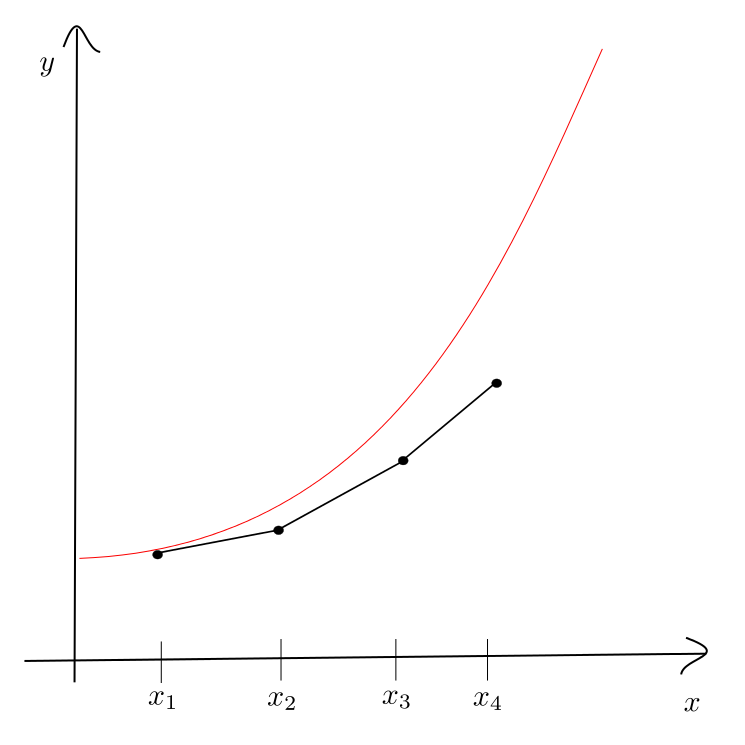
\includegraphics[scale=.3]{euler1}
  \end{flushleft}
  Find \( y_1 \text{ \& } y_{n+1} \) in general \\
  slope \( = f(x_0, y_0) \) \\
  \begin{flushleft}
    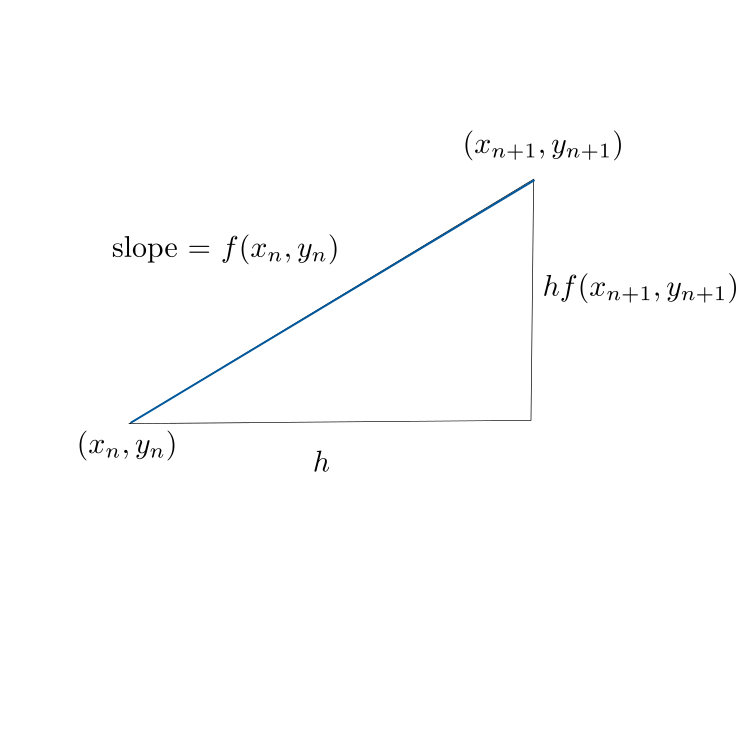
\includegraphics[scale=.3]{euler2}
  \end{flushleft}
  \( h = x_1-x_0 \)
  \[ y = f(x_0, y_0)(x-x_0) + y_0 \implies \]
  \[ y_1 = f(x_0, y_0)h + y_0 \]
  In general, 
  \[ \boxed{ y_{n+1} = hf(x_n,y_n) + y_n} \]
  Here
  \[ \boxed{ y_n \approx y(x_n)} \]
  % }}}

  % Date: 03.11.15 ------------------ {{{
  \newpage
  \marginpar{Date: 03.11.15 }
  Recall that an nth order linear ODE has the form 
  \[ 
  \tag{1} 
  \label{nth order linear ODE}
  y^{(n)} + \sum_{k=1}^n Pk(x)y^{(n-k)} = f(x)
  \]
  where \( Pk \) and \( f \) are cts for \( 1 \leq k \leq n \). \\
  The associated homogeneous nth order linear ODE to (1) is\\
  (2)
  \[ y^{(n)} + \sum_{k=1}^n Pk(x)y^{(n-k)} = 0 \]
  i.e., (1) with \( f(x) \equiv 0 \)\\
  Notation. put 
  \[ V = { y: I \to \mathbb{R} \text{ |  y has nth order derivative on I}  } \]
  then \( V \) is an \( \mathbb{R} \)- linear space. put 
  \[ W =  { y \in V \text{ | y is a soln to (2) }  } \]
  then the following holds\\[5mm]
  thrm. \( W \leq V \), i.e., the set of all solns to (2) is a linear
  space. \\
  Proof. If \( y \in W \) \& \( c \in \mathbb{R} \) then 
  \[ (cy)^{(n)} + \sum_{k=1}^n Pk(x)(cy)^{(n-k)}  = \]
  \[ (cy)^{(n)} + c\sum_{k=1}^n Pk(x)y^{(n-k)} \]
  \[ c(y^{(n)} + \sum_{k=1}^n Pk(x)y^{(n-k)}) \]
  \[ c \cdot 0 = 0 \]
  \( \therefore cy\in W \) \\
  If \( y_1, y_2 \in W \) then 
  \[ (y_1 + y_2)^{(n)} + \sum_{k=1}^n Pk(x)(y_1 +y_2 )^{(n-k)} = \]
  \[ y_1^{(n)} + \sum_{k=1}^n Pk(x)y_1^{(n-k)} + y_2^{(n)} +
  \sum_{k=1}^n Pk(x)y_2^{(n-k)} = \]
  \[ 0 + 0 = 0  \]
  \( \therefore y_1 + y_2 \in W \). Hence, \( W \in \mathbb{R} \)-linear
  subspace of V. \\[5mm]
  Recall: 
  Thrm (wronskian thrm). if \( f_1, ..., f_n \) are linearly independent
  in \( c^{(n-1)} (I) = \{ f:I\to \mathbb{R} \text{ | } f^{(n-1)} \text{
  is cts on I} \} \), then the wronskian of \( f_1, ..., f_n \) is identically 0
  for all \( x \in I \), i.e., for all \( x \in I \), 

  \[ |W(f_1, ...,f_n)(x)|  = det 
  \begin{pmatrix} 
    f_1(x)         & \cdots & f_n(x) \\
    f_1'(x)        & \cdots & f_n'(x) \\
    f_1''(x)       & \cdots & f_n''(x) \\
    \vdots         & \ddots & \vdots\\
    f_1^{(n-1)}(x) & \cdots & f_n^{(n-1)}(x) \\
  \end{pmatrix}
  =0\]


  Aside
  \[ A \vec{x}  = \vec{b} \]
  the soln space of 
  \[ A \vec{x} =\vec{0} \]
  is a linear space. the soln space of 
  \[ A \vec{x}  = \vec{b} \]
  is a affine linear space, with solns 
  \[ \vec{x} = \vec{x_0} + \vec{x_1}\]
  where \( \vec{x_0} \) is any hom soln

\section*{Exam 2}
  1. hom ODE \\
  2. ODE needing a subst to reduse to a 1st order linear/sep \\
  3. exact ODE \\
  4. population Model (logistic pop) \\
  5. population Model (havesting a logistic pop) \\ 
  % }}}

  % side stuff --------------- {{{
  %\section{Date: 02:18:2015}
  %Books \\
  %enderton "Mathematical logic" \\
  %kurnen "set theory" \\
  % Shellah's Archive
  % }}}

  %xy-pic
  %asymptote 


  \end{document}


\chapter{Third Test}

% vim:tw=72 sw=2 ft=tex
%         File: test3.tex
% Date Created: 2015 Mar 31
%  Last Change: 2015 Mar 31
%     Compiler: pdflatex
%       Author: joshua
\documentclass{article}
\usepackage{amsmath, amssymb}
\usepackage{amsthm}
\usepackage[utf8]{inputenc}
\usepackage[T1]{fontenc}
\usepackage[english]{babel}
\usepackage{graphicx}

\graphicspath{ {./images/} }

\usepackage{mathrsfs} % gives me a font I need
\usepackage[document]{ragged2e} % flush everything left dont wory about
% the error 

\DeclareMathOperator\arctanh{arctanh}
\DeclareMathOperator\sech{sech}

\newtheorem*{theorem}{Theorem}
\newtheorem*{corollary}{Corollary}

\theoremstyle{definition}
\newtheorem*{definition}{Definition}
\newtheorem*{example}{Example}

\begin{document}

% Date: 03.23.15 ------------------ {{{

%\marginpar{Date: 03.23.15 \\[5mm]
%\footnotesize{

%Aside \\
%Thrm( Wronskian Thrm). If \( \exists a \in I \) st det \( W(a) \neq 0
%\), then \( y_1, \dots , y_n \) (in \( \mathscr{D}^{(n-1)} (I) \)) are linearly
%independent, where 
%\[ 
%det W(a) =  
%\]
%\[  
%  \begin{vmatrix} 
%    y_1(x)         & \cdots & y_n(x) \\
%    y_1'(x)        & \cdots & y_n'(x) \\
%    y_1''(x)       & \cdots & y_n''(x) \\
%    \vdots         & \ddots & \vdots\\
%    y_1^{(n-1)}(x) & \cdots & y_n^{(n-1)}(x) \\
%  \end{vmatrix}
%\]

%}
%}
%\marginnote{this is some shit I guess you could say}
\begin{theorem}
  (Existence - Uniqueness Thrm, \( \exists \)! Thrm ). If I is an
  interval, \( a \in I \), and \( p_u \) for all \( 1 \leq k \leq n-1 \),
  and \( f \) are cts on \( I \), then 
  \( \forall b_i \), for \( 0 \leq i \leq n-1 \), (then initial value problem)  
\end{theorem}

\[ \text{ (1) } y^{(n)} + \sum_{k=1}^n y^{(n-k)} p_u(x) = f(x) \]
\& \( y^{(i)} (a) = b_i  \) , has a unique soln on \( I \). \\
Note: the solns to linear ODEs are unique on the whole interval \( I
\).\\[5mm]

\begin{theorem}
  Thrm. If \( w = \{ y \in \mathscr{D}^{(n)} (I) \text{ | } y \text{ satisfies (1)}
  \} \) then
  dim \( W \geq n \). \\[5mm]
\end{theorem}

\begin{proof}
  put \( y^{(i)}_j (a) = \delta_{ij} \),  where

  \[ 
  \delta_{ij} =
  \begin{cases}
    1, & \text{ if } i = j; \\
    0, & \text{ if } i \neq j
  \end{cases}
  \]

  for \( 1 \leq i \), \( j \leq n \). By the \( \exists \)! Thrm, for each
  \( j \) there is a unique soln to (1) on \( I \). Now, 

  \begin{align*}
    W(a) &= (y_j^{(i)}(a) ) \in \text{ Mat}_n( \mathbb{R}) \\
    &= I_n
  \end{align*}

  \[ \therefore |W(a)|=1 \neq 0 \]

  whence, \( y_1, \dots , y_n \) are linearly independent . Hence,

  \[ dim W \leq n  \]
\end{proof}

\begin{theorem}
  Thrm (Strong wronskian converse) If \( y_1, \dots , y_n \) are linearly
  independent ( in \( \mathscr{D}^{(n)} (I) \) ) and \( y_1, \dots , y_n
  \) are solns to 

  \marginpar{Date: 03.24.15 }

  \[ y^{(n)} + \sum_{k=1}^n y^{(n-k)} p_k(x) = 0 \]

  where \( p_k \) are cts on I for \( k=1, \dots , n \), then \( |W(a)
  \neq 0  \) for all \( a \in I \). 
\end{theorem}

%then \( \forall a \in I \), \(
%|W(a)| \neq 0 \). \\
\begin{proof}
  Assume that there is an \( a \in I \) st \( |W(a)| = 0 \), then
  the linear system 

  \[ \text{ (1) } W(a) \vec{x} = \vec{0} \]

  has a nontrivial soln, say \( \vec{x} = \vec{c} \in \mathbb{R}^n \)\\
  \( (W(a) \in \text{Mat}_n( \mathbb{R})) \). Denote: \( \vec{c} = (c_1,
  \dots , c_n) \neq \vec{0} \). \\[5mm]

  Put \( y = \sum_{j=1}^n c_j y_j \), then \( y \) satisfies (*) and % \in \mathscr{D}^{(n)}(I)\), then

  \[  y(a) = \sum_{j=1}^n c_j y_j(a) = 0  \implies\]

  \[ y'(a) = \sum_{j=1}^n c_j y'_j(a) = 0 \implies\]

  \[  y''(a) = \sum_{j=1}^n c_j y''_j(a) = 0  \implies\]

  \[ \vdots \]

  \[  y^{(n-1)}(a) = \sum_{j=1}^n c_j y^{(n-1)}_j(a) = 0 \text{ ( by(1)) } \]

  Notice that \( y \equiv 0 \) on \( I  \) also satisfies (*) and is such
  that \( y^{(k)}(a) = 0 \) for \( 1 \leq k \leq n-1 \). \( \therefore \)
  by \( \exists \)! thrm, 

  \[ \sum_{j=1}^n c_j y_j \equiv 0 \text{ on } I \]

  Thus, since \( y_1, \dots , y_n \) are lin ind, all \( c_j = 0 \), which
  is a contradiction.  
\end{proof}

\begin{theorem}
  If
  \[ W = \{ y \in \mathbb{R}^{(n)}(I) \text{ | } y \text{ satisfies (*) }  \}
  \]

  then dim \( W \leq n  \)
\end{theorem}

\begin{proof}
  let \( y_1, \dots , y_n \) be lin ind solns of (*); we show that
  there are scalars \( c_j \in \mathbb{R} \) st \( y = \sum_{j=1}^n
  c_jy_j\) on \( I \).

  Consider the linear system 

  \[ \text{ (2) } W(a) \vec{x} =
  \begin{pmatrix}
    y(a) \\
    y'(a) \\
    \vdots \\
    y^{(n-1)}(a)
  \end{pmatrix}\]

  where \( W(a) \) in the Wronskian matrix of \( y_1, \dots, y_n \). By
  the SWC, \( |W(a)| \neq 0 \). Thus, (2) has a unique, not-trivial soln,
  say \( \vec{0} \pm \vec{x} = \vec{c} \neq \vec{0} \in \mathbb{R}^n\). Thus

  \marginpar{Date: 03.25.15 }

  \[ W(a) \vec{c} =
  \begin{pmatrix}
    y(a) \\
    y'(a) \\
    \vdots \\
    y^{(n-1)}(a)
  \end{pmatrix}\]

  has rows 

  \begin{align*}
    \sum_{j=1}^n c_jy_j(a)         & = y(a) \\
    \sum_{j=1}^n c_jy'_j(a)        & = y'(a) \\
    \sum_{j=1}^n c_jy''_j(a)       & = y''(a) \\
    & \vdots \\
    \sum_{j=1}^n c_jy^{(n-1)}_j(a) & = y^{(n-1)}(a)
  \end{align*}

  Finally, since both \( y \) and \( \sum_{j=1}^nc_jy_j \) are solns to
  the hom nth order linear ODE (*) (the ODE being home and \( y_j \), for
  \( 1 \leq j \leq n \), being solns, so is any linear combo of \( y_j \)s
  since the soln space to a linear home ODE is linear) and both \( y \)
  and \(  \sum_{j=1}^nc_jy_j  \) satisfy all the same \( n \) many initial
  ?conbos?, by the \( \exists \)! thrm, \( y =  \sum_{j=1}^nc_jy_j  \) on
  \( I \). \( \therefore \) \( y \in \) Span \( \{ y_j \in W \text{ | } 1 \leq
  j \leq n \} \). Thus, dim \( W \leq n \).
\end{proof}

\begin{corollary}
  If 

  \[ W = \{ y \in D^{(n)} (I) \text{ | } y \text{ satisfies (x) } \} \]

  where

  \[ \text{ (*) } y^{(n)} + \sum_{k=1}^n y^{(n-k)} p_k(x) = 0 \]

  then dim \( W = n \).
\end{corollary}

\begin{proof}
  We showed that \( n \leq \text{ dim} W \leq n \).
\end{proof}

\begin{example}
  \( y'' - y = 0 \) \\
  Note that both \( y_1 = \cosh x \) and \( y_2 = \sinh x \) are solns on
  \( \mathbb{R} \). The soln space is \( 2 - \text{ dim'l } \). Not also
  that if 

  \[ a \cosh x + b \sinh x = 0 \text{ for all } x \in \mathbb{R} \]

  then in particular, \( x = 0 \implies a = 0 \).\\
  \( \therefore b \sinh x = 0 \) for all \( x \). \\

  However, if \( x \neq 0 \) then \( \sinh x \neq 0 \); whence, \( b = 0
  \). Hence, \( B = \{ \cosh x \text{ , } \sinh x \} \) are linearly
  independent solns to \( y'' = y \), and the soln space has dim'n 2, \( B
  \) is a basis for the soln space. \( \therefore \) every soln to \( y''
  = y\) has the form 

  \[ y = a \cosh x + b \sinh x \]

  for some \( a, b \in \mathbb{R} \). Likewise, \( B' = \{ e^x, e^{-x} \}
  \) is also a basis. Note:

  \[  |W(x)| = 
  \begin{vmatrix}
    e^x & e^{-x} \\
    e^x & -e^{-x} 
  \end{vmatrix}
  = e^x
  \begin{vmatrix}
    1 & e^{-x} \\
    1 & -e^{-x} 
  \end{vmatrix}
  =
  \begin{vmatrix}
    1 & 1 \\
    1 & -1 
  \end{vmatrix}
  = -2  \neq 0
  \]

  \( \therefore \) by Wronsky's Thrm, \( B' \) is lin ind. 
\end{example}

\begin{example}
  Example: \( y'' + y = 0 \) \\ 

  Here \( B = \{ \cos x, \sin x \} \) is a basis.
\end{example}

\underline{nth order hom linear ODEs with constant coefficients:}

\[ \text{ (1) } \sum_{k=0}^n a_ky^{(k)} = 0 \]

consider 

\[ y = e^{rx} \]

then 

\begin{align*}
  y'      & = re^{rx} = ry \implies \\
  y''     & = r^2e^{rx} = r^2y \implies \\
  & \vdots \\
  y^{(k)} & = r^ky
\end{align*}

thus, \( y = e^{rx} \) yields 

\begin{align*}
  0 & = \sum_{k=0}^n a_ky^{(k)} \\
  & = \sum_{k=0}^n a_kr^ky \\
  & = y\sum_{k=0}^n a_kr^{(k)}  \implies
\end{align*}

\[ \sum_{k=0}^n a_kr^{(k)} = 0 \]

\( \therefore y = e^{rx} \) is a soln to (1) if \( r \) is a root (zero)
of the char poly of \( \sum_{k=0}^n a_ky^{(k)} = 0 \), 

\marginpar{Date: 03.26.15 } % Continue notes  

\[ \rho (x) = \sum_{k=0}^n a_kx^k,\]
%which is called the caracteristic poly of (1) 

then \( y = e^{rx} \) is a soln to \( \sum_{k=0}^n a_ky^{(k)} = 0 \). 

\begin{example}
If \( r_1, \dots , r_n  \in \mathbb{R}\)  are paiswise distinct then \(
e^{r_1x}, \dots , e^{r_nx}\) are linearly independent (in \( \mathscr{F}
( \mathbb{R})\). we use the Wronskian: 

\[ |W(x)| = 
\begin{vmatrix}
  e^{r_1x} & e^{r_2x} & \cdots & e^{r_nx} \\
  r_1e^{r_1x} & r_2e^{r_2x} & \cdots & r_ne^{r_nx} \\
  \vdots & \vdots & \ddots & \vdots \\
  r_1^{n-1}e^{r_1x} & r_2^{n-1}e^{r_2x} & \cdots & r_n^{n-1}e^{r_nx} \\
\end{vmatrix}
\]

\[ 
e^{(r_1+r_2+ \cdots +r_n)x} =
\begin{vmatrix}
  1 & 1 & \cdots & 1  \\
  r_1 & r_2 & \cdots & r_n\\
  \vdots & \vdots & \ddots & \vdots \\
  r_1^{n-1} & r_2^{n-1} & \cdots & r_n^{n-1} \\
\end{vmatrix}
\]

\[ e^{(r_1+r_2+ \cdots +r_n)x} \prod_{1 \leq i < j \leq n}(r_j - r_i) \neq 0 \]

(for all \( x \) ). therefore by the wronskian thrm, \( e^{r_1x} ,
e^{r_2x}, \dots , e^{r_nx} \) ar lin ind, 
\end{example}

\begin{example}

(Vandermonds) \\
consider 
\[ 
V_n(x) = 
\begin{pmatrix}
  1 & x & x^2  & \cdots & x^{n-1} \\
  1 & r_2 & r_2^2 & \cdots & r_2^{n-1} \\
  1 & r_3 & r_3^2 & \cdots & r_3^{n-1} \\
  \vdots & \vdots & \vdots & \ddots  & \vdots \\
  1 & r_n & r_n^2 & \cdots & r_n^{n-1}
\end{pmatrix}
\]

which is an \( n \times n \) Vandermonde Matrix.\\
Put 

\[ f(x) = \det V_n(x) \in P_{n-1} \left[ \mathbb{R}\right],  \]

then \( f(r_j) = \det (V_n(r_j)) = 0 \) for all \( 2 \leq j \leq n \),
by the alternating property of determinates. therefore by the factor Thrm, 

\[ f(x) = a \prod\limits_{2 \leq j \leq n} (x-r_j) ,  \] % 2 \leq j \leq n

where 
\[ a = (-1)^{n-1}
\begin{vmatrix}
  1 & x & x^2  & \cdots & x^{n-1} \\
  1 & r_2 & r_2^2 & \cdots & r_2^{n-1} \\
  1 & r_3 & r_3^2 & \cdots & r_3^{n-1} \\
  \vdots & \vdots & \vdots & \ddots  & \vdots \\
  1 & r_n & r_n^2 & \cdots & r_n^{n-1}
\end{vmatrix}
,
\]

which is an \( (n-1) \times (n-1) \det \). therefore by the inductive
hypothesis, 

\[ a = (-1)^{n-1} \prod\limits_{2 \leq i < j \leq n}(r_j - r_i) \]

therefore 

\[ f(x) = (-1)^{n-1} \prod\limits_{2 \leq i < j \leq n} (r_j - r_i) \prod\limits_{2 \leq j \leq n} (x-r_j) \]

Notice that 
\[  \prod\limits_{2 \leq j \leq n}(x-r_j) = (-1)^{n-1}  \prod\limits_{2 \leq j \leq n}(r_j -x).  \]

Therefore

\begin{align*}
  f(x) &= (-1)^{n-1}  \prod\limits_{2 \leq i \leq j \leq n}(r_j-r_i)(-1)^{n-1}  \prod\limits_{2 \leq j \leq n}(r_j -x) \\
  &=  \prod\limits_{2 \leq j \leq n}(r_j -x)  \prod\limits_{2 \leq i
  \leq j \leq n} (r_j-r_i).  
\end{align*}

In particular, 

\begin{align*}
 \det V_n(r_1) &= f(r_1) \\
 &= \prod\limits_{2 \leq j \leq n}(r_j - r_1)  \prod\limits_{2 \leq j
 \leq i \leq n}(r_j-r_i) \\
 &= \prod\limits_{1 \leq i \leq j \leq n}(r_j - r_i).
\end{align*}

\end{example}

\marginpar{Date: 03.31.15 } % Continue notes 

Recall: the characteristic poly of \( \sum_{k=0}^n a_ky^{(k)} \) is 

\[ \rho (x) =  \sum_{k=0}^n a_kx^{(k)}  , \]

and we showed that if \( r_1, \dots , r_n \) are pairwise distinct then
\( B = \{ e^{r_1x}, \dots , e^{r_nx}\} \) is linearly independent (in \(
 \mathscr{C}^{( \infty )} (\mathbb{R})\) ). We also showed that if \( r \) is a
 zero of \( \rho (x) \) then \( y = e^{rx} \) is a soln to \(
 \sum_{k=0}^n a_ky^{(k)} = 0  \). This all immediatly implies the
 following: 

 \begin{theorem}
 If \(\rho (x)  \sum_{k=0}^n a_kx^{(k)} \) has \( n \) many distinct
 real zeros then  the soln space of 

 \[\text{(*) } \sum_{k=0}^n a_ky^{(k)}  = 0 \]

 has basis \( \{ e^{r_1x} , \dots , e^{r_nx}\} \), i.e., every soln of *
 has the form 

 \[ \sum_{j=1}^n c_je^{r_jx} . \]
 \end{theorem}

 \begin{example}
 (Revisited)

 Consider \( y'' - y = 0 \). This has char poly 
 \[ \rho (x) = x^2 -1 = (x-1)(x+1)  ,\]
 which has zeros \( \pm 1 \). 

 Thus, \( B = \{ e^x , e^{-x} \} \) is a basis for the soln space of 
 \[ y'' - y = 0  \]
 Q: What are the mising basis elements if a char poly has repeating
 zeros?

 \end{example}

 Recall the "ring" of polynomials 
 
 \[ \mathbb{R}[x] = \{ \sum_{k=0}^n a_kx^k \text{ | } n \in \mathbb{N}
 \text{ \& } a_k \in \mathbb{R} \} ,\]

 where

 \[ \sum_{k=0}^n a_kx^{(k)} + \sum_{k=0}^n b_kx^{(k)} = \sum_{k=0}^n
 (a_k + b_k)x^{(k)}   \]

 \[ \sum_{i=0}^m a_ix^{(i)} \sum_{j=0}^m b_jx^{(j)}  = \sum_{k=0}^{m+n}
 c_k x^{(k)}, \text{ where }\]

 \[ c_k = \sum_{i+j=k} a_ib_j .\]

 \underline{Notation}. Put \( D = \frac{d}{dx} \text{ : }
 \mathscr{C}^{(\infty)} (I)  \) 

 \( D^0 = i \) (identity on \(\mathscr{C}^{(\infty)} (I) \) ), and 

 \[ D^n = D D^{n-1} \text{ for } n \in \mathbb{Z}^+ .\]

 




\newpage
\section*{Books}
 Hausen and sullivan "Real Analysis" \\
 Reference: I.N. Herstein's "Topics in Abstract Algebra" (2nd ed),
 "Abstract Algebra" (3rd ed)\\
 Artin's "Algebra" \\
 (Formal poly : See hungerfords springer GTM.) \\


%the contropositive of \( A \implies B \) is 


%\marginpar{
%Aside \\

%Thrm( Wronskian Thrm). If \( \exists a \in I \) st det \( W(a) \neq 0
%\), then \( y_1, \dots , y_n \) (in \( \mathscr{D}^{(n-1)} (I) \)) are linearly
%independent, where 
%\[ 
%det W(a) =  
%\]




% }}}

\end{document}


\chapter{Fourth Test}

% vim:tw=72 sw=2 ft=tex
%         File: test4.tex
% Date Created: 2015 Apr 13
%  Last Change: 2015 May 06
%     Compiler: pdflatex
%       Author: joshua
\documentclass[12pt,a4paper]{article}
\usepackage{amsmath, amssymb}
\usepackage{amsthm}
\usepackage[utf8]{inputenc}
\usepackage[T1]{fontenc}
\usepackage[english]{babel}
\usepackage{graphicx}

\usepackage{mathrsfs} % gives me a font I need
\usepackage[document]{ragged2e} % flush everything left dont wory about
% the error 

\DeclareMathOperator\arctanh{arctanh}
\DeclareMathOperator\sech{sech}

\newtheorem*{theorem}{Theorem}
\newtheorem*{corollary}{Corollary}

\theoremstyle{definition}
\newtheorem*{definition}{Definition}
\newtheorem*{example}{Example}

\everymath{\displaystyle}

\begin{document}

\marginpar{Date: 04.13.15 } % Continue notes 
Here we address the possibility of the char poly \( \rho(x) \) of \(
\sum_{k=0}^{n} a_ky^{(k)} = 0  \) with complex zeros. So, assuming that
\( r = a + bi \) is a zero of \( \rho = \sum_{k=0}^{n} a_k x^k \), then
we know that \( y= e^{rk} = e^{(a+bi)x} = e^{ax} e^{(bx)i}\). Recall
that if \( a_k \in \mathbb{R} \) for \( 0 \leq k \leq n \), i.e., \(
\rho(x) \in \mathbb{R}[x] \), then \( \bar{r} = a-bi\) \( (b \pm 0 \) is
also a zero of \( \rho(x) \). Thus, in the case of \( r = a \pm bi \),
we are "missing" now not just one real-valued basis element, but two
real valued basis elements. 

Euler's identity enabels us to determine there two missing basis
elements: 

\[ \text{ (1) } e^{ix} = \cos(x) = i\sin(x) \in \mathbb{C} \text{ for all } x \in
\mathbb{R} \]

what led Euler to this identity are the Maclarin series: 

\[ e^x = 1 + \frac{x}{1!} + \frac{x^2}{2!} + \frac{x^3}{3!}+
\frac{x^4}{4!}+ \frac{x^5}{5!} + \cdots = \sum_{n \geq 0} \frac{x^n}{n!};\]

\[ \cos(x) = 1 - \frac{x^2}{2!} +
\frac{x^4}{4!} - \frac{x^6}{6!} + \frac{x^8}{8!} - \frac{x^10}{10!} +
\cdots = \sum_{n \geq 0} (-1)^n \frac{x^{2n}}{2n!};\]

\[ \sin(x) =  x -  \frac{x^3}{3!} + \frac{x^5}{5!} - \frac{x^7}{7!} +
\frac{x^9}{9!} - \frac{x^11}{11!} + \cdots = \sum_{n \geq 0} (-1)^n
\frac{x^{2n +1}}{(2n+1)!};\]

These hold for all \( x \in \mathbb{R} \). Notice that (1) simply gives
pts on the unit circle in \( \mathbb{C} \)

\[ |e^{ix}| = 1 \text{ for all } x \in \mathbb{R} \]

Note: \( e^{i \pi} + 1 = 0. \) \( (x = \pi) \)

Observe that \( e^{ix} \) is a complex-valued scalar mult of \( \cos x
\) \& \( \sin x \). So, back to the soln

\begin{align*}
  y &= e^{ax} e^{(bx)i} \\
  &=e^{ax}(\cos bx + i \sin bx) \\
  &= e^{ax} \cos x + i(e^{ax} \sin bx),
\end{align*}

which is likewise a complex-valued linear combo of \( e^{ax} \cos bx \) \& \(
e^{ax} \sin bx \). These are to real-balued soln to the ODE \(
\sum_{k=0}^{n}a_ky^{(k)} =0, \) i.e., there are the two missing basis
elements. therefore if \( (x-r)^m, \) where \( r = a +bi \), is a factor
of \( \rho(x) \), then the corespoinding basis elements are: 

\begin{align*}
  e^{ax} \cos bx &\text{ , } e^{ax} \sin bx \\
  xe^{ax} \cos bx &\text{ , } xe^{ax} \sin bx \\
  x^2e^{ax} \cos bx &\text{ , } x^2e^{ax} \sin bx \\
  \vdots & \vdots  \\
  x^{m-1}e^{ax} \cos bx &\text{ , } x^{m-1}e^{ax} \sin bx
\end{align*}

Here there are the missing 2m many basis elements. 

\marginpar{Date: 04.14.15 } % Continue notes 

\begin{example}
  \[ y'' + y' - y = \sin^2x \]
  Here \( \sum_{k=0}^{n} y^{(k)} = f(x) \), where \( n=2 \) and \( f(x) =
  \sin^2x\). Notice that 

  \begin{align*}
    y &= \sin^2x \implies \\
    y' &= 2 \sin x \cos x \implies \\
    y'' &= 2 \cos^2x - 2\sin^2x.
  \end{align*}

  \begin{align*}
    y &= \sin^2x; \\
    y' &= 2 \sin x \cos x = \sin 2x \\
    y'' &= 2 \cos^2x - 2\sin^2x = 2 \cos 2x.
  \end{align*}

  the terms in there derivatives are 

  \begin{align*}
    1, \\
    \sin^2x, \\
    \sin x \cos x \\
    \cos^2x. 
  \end{align*}

  Another way to see these terms is as 

  \begin{align*}
    1, \\
    \cos 2x \\
    \sin 2x. 
  \end{align*}

  We consider a posible particular soln 

  \[ y_p = a + b\cos 2x + c \sin 2x, \]

  which is a linear combo of the terms above. Note that \( y_p \) is a
  particular soln iff 

  \[ y_p'' + y_p' - y_p = \sin^2x \]

  Now, 

  \begin{align*}
    y_p &= a + b\cos 2x + c \sin 2x \implies \\
    y_p' &= -2b\sin2x + 2c\cos2x \implies \\
    y_p'' &= -4b\cos2x -4c\sin2x \implies
  \end{align*}

  \[ y_p'' + y_p' - y_p = \sin^2x \iff \]

  \[ (2c-4b)\cos2x - (2b+4c)\sin2x - b\cos2x -c\sin2x -a = \sin^2x \iff \]
  \[ (2c-5b)\cos2x - (2b+5c)\sin2x -a = \frac{1-\cos2x}{2} \iff \]
  \[ -a-1/2+(2c-5b+1/2)\cos2x - (2b+5c)\sin2x = 0. \]

  This last equation is an identity if 

  \[ a = -1/2 \text{ \& } 
  \begin{cases}
    -5b + 2c + 1/2 &= 0 \\
    2b + 5c &=0.
  \end{cases}
  \]

  Note:
  \[
  \begin{cases}
    -10b + 4c &= -1 \\
    2b + 5c &= 0
  \end{cases}
  \]
  \[
  \begin{bmatrix}
    10 & 25 & | & 0 \\
    -10 & 4 & | & -1 \\
  \end{bmatrix}
  \]

  \begin{align*}
    c &= -1/29 \\
    b &= 5/58
  \end{align*}

  Therefore

  \[ y_p = -1/2 + \frac{5}{58} \cos2x - \frac{1}{29}\sin2x, \]

  Which you have cheked is an actual soln to \( y'' + y' -y = \sin^2x. \)

\end{example}

\marginpar{Date: 04.15.15 } % Continue notes 

\begin{example}
  \[ y'' + y' - y = \sec x \]

  \begin{align*}
    f(x) &= \sec x \\
    f'(x) &= \sec x \tan x \\
    f''(x) &= \sec x \tan^2x + \sec^3x \\
    &= \sec x (\sec^2x - 1) + \sec^3x \\
    &= 2\sec^3x - \sec x
  \end{align*}

  Put 

  \[ B = \{ 1, \sec x, \sec x \tan x, \sec^3x \}  \]

  Also, put 

  \[ y_p = a + b \sec x + c\sec x \tan x + d \sec^3x \]

  \[ y_p'  \]

  Since \( \sec^3x \tan x \notin  \) Span \( B \), the method of
  undetermined coefis fails. \\[5mm]

  Idea: Consider \( B = \{ y_1, \dots, y_n \} \), the basis of \(
  \sum_{k=0}^{n} a_k y^{(k)} = 0 \), and 

  \[ \text{ (1) } y_p = \sum_{k=1}^{n} v_k(x) y_k(x). \]

  We will show that a particular soln of \( \sum_{k=0}^{n} a_k y^{(k)}
  = f(x)  \) always has form (1) for some \( v_k(x) \in C^{(n)} (I) \).
  this is called " Variation of parameters."

\end{example}

\marginpar{Date: 04.16.15 } % Continue notes 

We want a particular soln \( y = v_1(x) y_1(x) + v_2(x) y_2(x) \) to \(
\sum_{k=1}^{2} a_k y^{(k)} = f(x) \), where the hom soln space has basis
\( B = \{ y_1, y_2 \}  \subset C^{(2)}(I) \). Here we require 

\[  y_p'' + py_p' + qy_p = f(x) \text{ (monic). } \]

\[ y_p = v_1y_1 + v_2y_2 \implies \]

\[ y_p' = v_1'y_1 + v_1y_1' + v_2'y_2 + v_2y_2' \]

If \( v_1'y_1 + v_2'y_2 = 0 \) then 

\[ y_p' = v_1y_1' + v_2y_2' \]

Thus, 

\[ y_p'' = v_1'y_1' + v_1y_1'' + v_2'y_2' v_2y_2'' \]

\[ y_p'' +py_p' + qy_p = f(x) \iff \]

\[ v_1'y_1' + v_1y_1'' + v_2'y_2' v_2y_2'' + pv_1y_1' + pv_2y_2' +
qv_2y_1 + qv_2y_2 = f(x) \iff \]

\[ v_1(y_1'' + py_1' + qy_1) + v_2(y_2'' + py_2' + qy_2) + v_1' y_1' +
v_2'y_2' = f(x) \iff \]

\[ v_1'y_1' + v_2'y_2' = f(x). \]

therefore

\begin{cases}
  y_1' v_1' + y_1'v_2' = f(x) \\
  y_1v_1' + y_2v_2' = 0
\end{cases}

iff 

\[ 
\begin{pmatrix}
  y_1 & y_2 \\
  y_1'& y_2' 
\end{pmatrix}
\begin{pmatrix}
  v_1'\\
  v_2' 
\end{pmatrix}
=
\begin{pmatrix}
  a\\
  b
\end{pmatrix}
\]

% missed some stuff

Therefore 

\[ v_1 = - \int \frac{y_2(x)f(x)}{|w(x)|} dx \]

and 

\[  v_2 =  \int \frac{y_1(x)f(x)}{|w(x)|} dx \]

Hence, 

\[ y_p(x) =  \]

% missed some more stuff

Now, in general, consider 

\[ \sum_{k=0}^{n} a_ky^{(k)} = f(x) \]
with basis \( B = \{ y_j \in C^{(n)} (I) | 1 \leq j \leq n \} \) for the
assoc hom ODE. Also, consider 

\[ y_p= \sum_{j=1}^{n} v_jy_j, \]
then
\begin{align*}
  y_p' &= \sum_{j=1}^{n}(v_j'y_j +v_jy_j') \\
  &= \sum_{j=1}^{n} v_jy_j' \text{ , if } \sum_{j=1}^{n}v_j'y_j = 0.
\end{align*}

Now, 

\begin{align*}
  y_p'' &= \sum_{j=1}^{n}(v_j'y_j' + v_jy_j'') \\
  &= \sum_{j=1}^{n}y_jy_j'' \text{ , if } \sum_{j=1}^{n}v_j'y_j' =0
\end{align*}

continuing, 

\[ y_p^{(k)} = \sum_{j=1}^{n} v_jy_j^{(k)} \text{ , if }
\sum_{j=1}^{n}v_j'y_j^{(k-1)} =0 \]

for \( 1 \leq k \leq n-1 \). Finally, 

\begin{align*}
  y_p^{(n)} &= \sum_{j=1}^{n} (v_j'y_j^{(n-1)} +v_jy_j^{(n)}) \\
  &=    \sum_{j=1}^{n} v_j'y_j^{(n-1)} + \sum_{j=1}^{n}v_jy_j^{(n)}) 
\end{align*}

Therefore

\[ \sum_{k=1}^{n}a_ky_p^{(k)} = f(x) \iff \]

\[ a_n \sum_{j=1}^{n} v_j'y_j^{(n-1)} + a_n  \sum_{j=1}^{n}v_jy_j^{(n)}
+ \sum_{k=1}^{n-1}a_k \sum_{j=1}^{n}v_jy_j^{(k)} = f(x) \iff\]

\[  a_n \sum_{j=1}^{n} v_j'y_j^{(n-1)} +  \sum_{j=1}^{n} a_nv_jy_j^{(n)}
+ \sum_{j=1}^{n} \sum_{k=1}^{n=1} a_kv_jy_j^{(k)} = f(x) \iff
\]

\[ 
a_n \sum_{j=1}^{n} v_j'y_j^{(n-1)}  + \sum_{j=1}^{n}v_j \sum_{k=1}^{n}
a_ky_j^{(k)} = f(x) \iff
\]

\[ a_n \sum_{j=1}^{n} v_n'y_j^{(n-1)} = f(x) \]

since \( y_j \in B. \) Thus, 

\begin{align*}
  \sum_{j=1}^{n}v_j'y_j &= 0  \text{ 1st eqn }\\
  \sum_{j=1}^{n}v_j'y_j' &= 0 \text{ 2nd eqn }\\
  \vdots \\
  \sum_{j=1}^{n}v_j'y_j^{(k-1)} &= 0 \text{ kth eqn }\\
  \vdots \\
  \sum_{j=1}^{n}v_j'y_j^{(n-2)} &= 0 \text{ (n-1)th eqn }\\
  a_n\sum_{j=1}^{n}v_j'y_j^{(n-1)} &= f(x) \text{ nth eqn }\\
\end{align*}





Now, 
\begin{align*}
  y_p' &= v_1'y_1 + v_1y_1' + v_2'y_2 + v_2y_2' \implies \\
  y_p'' &= v_1''y_1 + v_1'y_1' + v_1'y_1' + v_1y_1'' + 
  v_2''y_2 + v_2'y_2' + v_2'y_2' + v_2y_2'' \\
  &= 2(v_1'y_1' + v_2'y_2') + v_1y_1'' + v_2y_2'' ,  
\end{align*}

if we impose the condition \( v_1''y_1 + v_2''y_2 = 0. \) therefore 

\begin{align*}
  f(x) &= y_p'' + py_p' + qy_p \\
  &= 2(v_1'y_1' + v_2'y_2') + v_1y_1'' + v_2y_2'' +
  pv_1'y_1 + pv_1y_1' + pv_2'y_1 _ pv_2y_2' + q_vy_1 + qv_2y_2\\
  &= v_1(y_1'' + py_1' +qy_1) + v_2(y_2'' + py_2' +qy_2) + 2(v_1'y_1' +
  v_2'y_2') + p(v_1'y_1'+v_2'y_2) \\
  &= 2(v_1'y_1' + v_2'y_2') + p(v_1'y_1 + v_2'y_2)
\end{align*}

therefore, 

\[ f(x) =  2(v_1'y_1' + v_2'y_2') + p(v_1'y_1 + v_2'y_2)
\]

implies 

\[ f(x) = v_1'(2y_1' +py_1) + v_2'(2y_2' +py_2) \]


% Date: 04.20.15 ------------------ {{{
\newpage
\marginpar{Date: 04.20.15 }

We want a particular soln \( y = v_1(x) y_1(x) + v_2(x) y_2(x) \) to \(
\sum_{k=1}^{2} a_k y^{(k)} = f(x) \), where the hom soln space has basis
\( B = \{ y_1, y_2 \}  \subset C^{(2)}(I) \). Here we require 

\[  y_p'' + py_p' + qy_p = f(x) \text{ (monic). } \]

\[ y_p = v_1y_1 + v_2y_2 \implies \]

\[ y_p' = v_1'y_1 + v_1y_1' + v_2'y_2 + v_2y_2' \]

If \( v_1'y_1 + v_2'y_2 = 0 \) then 

\[ y_p' = v_1y_1' + v_2y_2' \]

Thus, 

\[ y_p'' = v_1'y_1' + v_1y_1'' + v_2'y_2' v_2y_2'' \]

\[ y_p'' +py_p' + qy_p = f(x) \iff \]

\[ v_1'y_1' + v_1y_1'' + v_2'y_2' v_2y_2'' + pv_1y_1' + pv_2y_2' +
qv_2y_1 + qv_2y_2 = f(x) \iff \]

\[ v_1(y_1'' + py_1' + qy_1) + v_2(y_2'' + py_2' + qy_2) + v_1' y_1' +
v_2'y_2' = f(x) \iff \]

\[ v_1'y_1' + v_2'y_2' = f(x). \]

therefore

\[
\begin{cases}
  y_1' v_1' + y_1'v_2' = f(x) \\
  y_1v_1' + y_2v_2' = 0
\end{cases}
\]

iff 

\[ 
\begin{pmatrix}
  y_1 & y_2 \\
  y_1'& y_2' 
\end{pmatrix}
\begin{pmatrix}
  v_1'\\
  v_2' 
\end{pmatrix}
=
\begin{pmatrix}
  a\\
  b
\end{pmatrix}
\]

% missed some stuff

Therefore 

\[ v_1 = - \int \frac{y_2(x)f(x)}{|w(x)|} dx \]

and 

\[  v_2 =  \int \frac{y_1(x)f(x)}{|w(x)|} dx \]

Hence, 

\[ y_p(x) =  \]

% missed some more stuff

Now, in general, consider 

\[ \sum_{k=0}^{n} a_ky^{(k)} = f(x) \]
with basis \( B = \{ y_j \in C^{(n)} (I) | 1 \leq j \leq n \} \) for the
assoc hom ODE. Also, consider 

\[ y_p= \sum_{j=1}^{n} v_jy_j, \]
then
\begin{align*}
  y_p' &= \sum_{j=1}^{n}(v_j'y_j +v_jy_j') \\
  &= \sum_{j=1}^{n} v_jy_j' \text{ , if } \sum_{j=1}^{n}v_j'y_j = 0.
\end{align*}

Now, 

\begin{align*}
  y_p'' &= \sum_{j=1}^{n}(v_j'y_j' + v_jy_j'') \\
  &= \sum_{j=1}^{n}y_jy_j'' \text{ , if } \sum_{j=1}^{n}v_j'y_j' =0
\end{align*}

continuing, 

\[ y_p^{(k)} = \sum_{j=1}^{n} v_jy_j^{(k)} \text{ , if }
\sum_{j=1}^{n}v_j'y_j^{(k-1)} =0 \]

for \( 1 \leq k \leq n-1 \). Finally, 

\begin{align*}
  y_p^{(n)} &= \sum_{j=1}^{n} (v_j'y_j^{(n-1)} +v_jy_j^{(n)}) \\
  &=    \sum_{j=1}^{n} v_j'y_j^{(n-1)} + \sum_{j=1}^{n}v_jy_j^{(n)}) 
\end{align*}

Therefore

\[ \sum_{k=1}^{n}a_ky_p^{(k)} = f(x) \iff \]

\[ a_n \sum_{j=1}^{n} v_j'y_j^{(n-1)} + a_n  \sum_{j=1}^{n}v_jy_j^{(n)}
+ \sum_{k=1}^{n-1}a_k \sum_{j=1}^{n}v_jy_j^{(k)} = f(x) \iff\]

\[  a_n \sum_{j=1}^{n} v_j'y_j^{(n-1)} +  \sum_{j=1}^{n} a_nv_jy_j^{(n)}
+ \sum_{j=1}^{n} \sum_{k=1}^{n=1} a_kv_jy_j^{(k)} = f(x) \iff
\]

\[ 
a_n \sum_{j=1}^{n} v_j'y_j^{(n-1)}  + \sum_{j=1}^{n}v_j \sum_{k=1}^{n}
a_ky_j^{(k)} = f(x) \iff
\]

\[ a_n \sum_{j=1}^{n} v_n'y_j^{(n-1)} = f(x) \]

since \( y_j \in B. \) Thus, 

\begin{align*}
  \sum_{j=1}^{n}v_j'y_j &= 0  \text{ (1st eqn) }\\
  \sum_{j=1}^{n}v_j'y_j' &= 0 \text{ (2nd eqn) }\\
  \vdots \\
  \sum_{j=1}^{n}v_j'y_j^{(k-1)} &= 0 \text{ (kth eqn) }\\
  \vdots \\
  \sum_{j=1}^{n}v_j'y_j^{(n-2)} &= 0 \text{ ((n-1)th eqn) }\\
  a_n\sum_{j=1}^{n}v_j'y_j^{(n-1)} &= f(x) \text{ (nth eqn) }\\
\end{align*}

\[ \implies W(y_j)_{1 \leq j \leq n} 
\begin{pmatrix}
  v_1'\\
  \vdots \\
  v_n'
\end{pmatrix}
=
f(x) \vec{e_n}
\]

Notice that \( |W(y_j)_{1 \leq j \leq n}| \neq 0 \) for all \( x \in I
\) since \( y_js \) are linearly independent  ( being that \( y_j \in B
\)). Thus, by Cramer's Rule, 

\[ v_j' = \frac{D_j}{D},  \]

where \( D = |W(y_j)_{1 \leq j \leq n}| \) and

\[ D_j =
\begin{vmatrix}
  y_1 & \cdots & 0 & \cdots & y_n \\
  y_1' & \cdots & 0 & \cdots & y_n' \\
  y_1'' & \cdots & 0 & \cdots & y_n'' \\
  \vdots &       & \vdots & & \vdots \\
  y_1^{(n-1)} & \cdots & f(x) & \cdots & y_n^{(n-1)}
\end{vmatrix}
= (-1)^{n+j} f(x) |W_{n-1} (y_k)_{\substack{1 \leq k \leq n \\ j \neq
k}}| 
\]

Therefore 

\[ v_k' = (-1)^{j+n}f(x) \frac{|W_{n-1}(y_k)_{\substack{1 \leq k \leq n
\\
j \neq k}}|}{a_n|W_n(y_k)_{1 \leq k \leq n}|}  \]

Thus, 

\[ \text{ (1) } v_k(x) = 
\frac{(-1)^{j+n}}{a_n} \int f(x) \frac{|W_{n-1}(y_k)_{\substack{1 \leq
k \leq n \\
j \neq k}}|}{a_n|W_n(y_k)_{1 \leq k \leq n}|}  dx,
\]

Where \( y_p(x) = \sum_{k=1}^{n}v_k(x)y_k(x) \) is a particular soln to
\( \sum_{k=1}^{n}a_ky^{(k)} = f(x) \). (1) is called the variation of
parameters formulas. \\[5mm]

Ch 4 systems of ODEs 

\begin{example}
  Consider a curve \( \vec{r}:[a,b] \to \mathbb{R}^n \), where \(
  \vec{r}(t) = (x_1(t), \dots , x_n(t)) \) and \( t \in [a,b] \). By
  Newton's 2nd Law, \( \vec{F} = m\vec{a} = m\vec{r}''(t)\). Thus, 

  \[ 
  \begin{pmatrix}
    m(t)x_1''(t) \\
    m(t)x_2''(t) \\
    \vdots \\
    m(t)x_n''(t) 
  \end{pmatrix}
  =
  \begin{pmatrix}
    F_1(t) \\
    F_2(t) \\
    \vdots \\
    F_n(t) 
  \end{pmatrix}
  ,
  \]

  which is a system of \( n \) many 2nd order ODEs in \( (x_1, \dots ,
  x_n) \)


\end{example}



% }}}

\marginpar{Date: 04.21.15 } % Continue notes 

\marginpar{Date: 04.22.15 } % Continue notes 

\begin{example}
  Consider an 

  \[ \text{ (1) } y^{(n)}+ \sum_{k=0}^{n-1} p_k(x) = f(x), \]

  \[ y^{(n)} + p_{n-1}y^{(n-1)} + \cdots + p_2(x)y'' + p_1(x)y' +
  p_0(x)y = f(x). \]

  put \(y_k = y^{(k-1)}  \) for \( 1 \leq k \leq n+1 \), then 

  \begin{align*}
    y_1 &= y \implies \\
    y_2 &= y' = y_1' \implies \\
    y_3 &= y'' = y_1'' = y_2' \implies \\
    y_4 &= y''' = y_1''' = y_2'' = y_3'  \implies \\
    &\vdots \\
    y_{n+1} &= y^{(n)} = y_n'
  \end{align*}

  Thus, (1) becomes 

  \[ \text{ (2) } y_n' + \sum_{k=0}^{n-1}p_k(x)y_k' = f(x), \]

  which is a first order linear ODE. puting (2) whith the alone n-1
  many 1st order ODEs yields the following 1st order system: with n
  many ODEs:

  \[
  \begin{cases}
    y_n' + \sum_{k=0}^{n-1}p(x)y_k' = f(x)  \\
    y_1' = y_2 \\
    y_2' = y_3 \\
    \vdots \\
    y_{n-1}' = y_n
  \end{cases}
  \]

  Again, this is a system of n many 1st linear ODEs from a single nth
  order linear ODE. This gives yet another example to motivate studying
  systems of linear ODEs.

\end{example}

\begin{example}
  page 255 number 12 \\ 

  \[ 
  \begin{cases}
    x' = y  \\
    y' = x 
  \end{cases}
  \]

  Note: \( x = y' = x'' \). So, this yields \( x'' - x = 0 \), which has
  basis \( B = \{ \cosh t, \sinh t \} \). Thus, 

  \[ x = a \cosh t + b \sinh t \]

  Now, 

  \[ y =  b \cosh t + a \sinh t\]

  Notice that if \( \vec{r}(t) = (x(t), y(t))  \) then \( \vec{r}'(t) =
  (x'(t), y'(t)) = (y(t), x(t))  \). We want such an \( \vec{r}(t)  \). In otherwords,
  we may view the above system as a single. 1st order ODE of a
  parametric function. 

  Recall that 

  \[ \cosh (\alpha + t) = \cosh \alpha \cosh t + \sinh \alpha \sinh t \]

  Take \( A \in \mathbb{R} \) st \( a/A \geq 1 \), then \( a/A \in \)
  Range \( (\cosh)\). Now, we want \( \alpha \in \mathbb{R} \) st

  \[ a = A \cosh \alpha \text{ \& }  b = A \sinh \alpha.\]

  So, 

  \( \coth \alpha = \frac{ \cosh \alpha}{ \sinh \alpha} = \frac{a}{b} \)
  holds for some \( \alpha \) st \( |\alpha| < 1 \) since \( \text{
  Range} (\coth) = \mathbb{R} \). therefore for this \( \alpha \), 

  \begin{align*}
    x &=  a \cosh t + b \sinh t \\
    &= A \cosh \alpha \cosh t + A \sinh \alpha \sinh t \\
    &= A \cosh (\alpha + t).
  \end{align*}

  therefore \( x = A \cosh (\alpha + t) \); whence, \( y = x' = A \sinh
  (\alpha + t).\)

  Hence, 

  \[ x^2 - y^2 = A^2 \implies \frac{x^2}{A^2} - \frac{y^2}{A^2} = 1 \]

  These are the solns to \( \vec{r}'(t) = (x'(t), y'(t)).  \) Note : \(
  \text{ Range} (\cosh) = [1,\enfinity)\). So, if \( A > 0 \) then \( x(t)
  > 0\); where, \( \vec{r}(t) \) coresponds to the righthand branch.
  Whereas, if \( A<0 \) then \( \vec{r}(t) \) coresponds to the left hand
  branch. 

  Notice that we soved this linear system by "substitution." 

\end{example}

\marginpar{Date: 04.23.15 } % Continue notes 

\begin{example}
  (Recall). 

  let \( \vec{r}(t) = (x(t), y(t))\), and consider \( \vec{r}'(t) =
  (x'(t), y'(t)) \), then 

  \[
  \begin{cases}
    x'(t) = y(t) \\
    y'(t) = x(t)
  \end{cases}
  \iff
  \begin{cases}
    x'(t) - y(t) =0 \\
    y'(t) - x(t) =0
  \end{cases}
  \iff
  \begin{cases}
    L_{11}x + L_{12}y = 0 \\
    L_{21}x + L_{22}y = 0
  \end{cases}
  \iff
  \]

  \[
  \begin{pmatrix}
    L_{11} & L_{12} \\
    L_{21} & L_{22}
  \end{pmatrix}
  \begin{pmatrix}
    x \\
    y
  \end{pmatrix}
  = 
  \vec{0}
  \]

  Where \( L_{11} = D = L_{22} \) and \( L_{12} = -1 = L_{21} \) 

  In other symbols, 

  \[ 
  \begin{pmatrix}
    D & -1 \\
    -1 & D
  \end{pmatrix}
  \begin{pmatrix}
    x \\
    y
  \end{pmatrix}
  = 
  \vec{0}
  \]

  Recall that \( \mathbb{R}[D] \equiv \mathbb{R}[x]; \) in particular,
  \( \mathbb{R}[D] \) is communative "ring" (multiplicative
  communative).

  Solve by "elimination:"

  \[ L_{21}(L_{11}x + L_{12}y) = L_{21}0 \implies \]

  \[ L_{21}L_{11}x + L_{21}L_{12}y = L_{21}0 \]

  \[ L_{11}(L_{21}x + L_{21}y) = L_{11}0 \implies  \]

  \[ L_{11}L_{21}x + L_{11}L_{21}y = 0 \]

  \hline

  \[ L_{21}L_{12}y - L_{11}L_{22}y = 0 \implies \]

  \[ (L_{21}L_{12} - L_{11}L_{22}) y= 0 \implies \]

  \[ 
  \begin{vmatrix}
    L_{11} & L_{12} \\
    L_{21} & L_{22}
  \end{vmatrix}
  y
  = 0
  \]

  Anologosly 


  \[ 
  \begin{vmatrix}
    L_{11} & L_{12} \\
    L_{21} & L_{22}
  \end{vmatrix}
  x
  = 0
  \]

  Therefore

  \[ ( |L|I) 
  \begin{pmatrix}
    x \\
    y
  \end{pmatrix}
  = \vec{0}
  \]

  where

  \[
  L=
  \begin{pmatrix}
    L_{11} & L_{12} \\
    L_{21} & L_{22}
  \end{pmatrix}
  \]

  Recall: If A is a sq matrix then 

  \[ AA^a = |A|I \]

  This holds for any A over a commutative ring, e.g., 

  \[ A \in \text{ Mat }_n(R) \]

  where R is a commutative ring say \( R = \mathbb{C} \)

  Thus if \( L \in \text{ Mat}_n( \mathbb{R}[D]) \) then 

  \[ L^aL = |L|I_n, \]

  where \( I_n \text{ Mat}_n( \mathbb{R}[D]),  \)

  \[ 
  I_n = 
  \begin{pmatrix}
    1 & \cdots & 0 \\
    \vdots &  & \vdots \\
    0 & \cdots & 1
  \end{pmatrix}
  \text{ , \& }
  1_{Id} \in \mathbb{R}[D]
  \]

  consider \( L \in \text{ Mat}_n( \mathbb{R}[D]), \) \\

  \( \vec{x}(t) = (x_1(t), \dots , x_n(t)) \), \( \vec{F}(t) = (F_1(t),
  \dots, F_n(t)) \in (C^{(d)}(I))^n,\) where \( d= \text{ max} \{ \text{
  deg }(L_{ij}) \text{ | } 1 \leq i \text{ , } j \leq n \} \) and \( L =
  (L_{ij}),  \) and the system of linear ODEs

  \[ \text{ (1) }
  L \vec{x} = \vec{F} \iff 
  \begin{pmatrix}
    L_{11} & L_{12} & \cdots L_{1n} \\
    L_{21} & L_{22} & \cdots L_{2n} \\
    \vdots & \\
    L_{n1} & L_{n2} & \cdots L_{nn} 
  \end{pmatrix}
  \begin{pmatrix}
    x_1(t) \\
    x_2(t) \\
    \vdots \\
    x_n(t)
  \end{pmatrix}
  =
  \begin{pmatrix}
    F_1(t) \\
    F_2(t) \\
    \vdots \\
    F_n(t)
  \end{pmatrix}
  \]

  Here 

  \[ L_{ij} = \sum_{k=0}^{m_{ij}} a_{i_k j_k} D^k \in \mathbb{R}[D] \]

  Applying the adjoint formula to (1) 

  \[ \text{ (2) } (|L|I_n) \vec{x} = L^a \vec{F}. \]

  Recall: \( A^a = (c_{ij})^T \), \( C_{ij} = (-1)^{i+j} |M_{ij}| \)

  In component form, (2) says that 

  \[ \text{ (3) } |L|x_i(t) = _i(L^a) \vec{F}(t) ,\]

  where \( _i(L^a) \) is the ith row of \( L^a \). Notice that (3) is a
  linear ODE in the single unknown funct \( x_i(t) \). therefore previous
  methods can be used to solve (3). 
\end{example}

\marginpar{Date: 04.27.15 } % Continue notes 

Now, we consider first order linear systems, at first, without constant
coefficients. These have the form 

\[ \vec{x}'(t) + p(t) \vec{x}(t) = \vec{q}(t),  \]

where \( \vec{x}: I \subseteq \mathbb{R} \to \mathbb{R}^n \) and \( p(t)
\in \text{ Mat}_n (C(I)) \) and \( \vec{q} \in ( C^{(1)}(I))^n \). 

In "normal form" this becomes 

\[   \vec{x} \;'(t) = p(t) \vec{x}(t) + \vec{q}(t) \]



Aside: \( R[D] \) is a communative "ring." however, \( (C(t))[D] \) this
is not a communative, the point is that to use the det proputies
developed last semester, we need \( \text{ Mat}_n( \mathbb{R}) \), where
\( \mathbb{R} \) is commutative ring (then thos proff genral

\begin{example}
  (\( ((C)(I))[D] \) is not commutative). 

  Put

  \[ L_1 = -tD+1 \]
  \[ L_2 = t^2D - 3, \]

  then \( L_1, L_2 \in ( C^{(\infty)}( \mathbb{R}) ) [D] \). Notice that 

  \begin{align*}
    L_2x &= (t^2D-3)x \\
    &= t^2Dx-3x \\
    &= t^2x' -3x \implies
  \end{align*}

  \begin{align*}
    L_1L_2x &= (-tD + 1)L_2x \\
    &= (-tD + 1)(t^2Dx-3x) \\
    &= -tD(t^2Dx-3x) + t^2Dx-3x \\
    &= -tD(t^2Dx) + 3tDx + t^2Dx-3x \\
    &= -t(2tDx + t^2D^2x) + 3+ Dx + t^2Dx-3x \\
    &= -2t^2Dx - t^3D^2x + 3tDx + t^2Dx - 3x \\
    &= -t^2Dx - t^3D^2x + 3tDx - 3x. 
  \end{align*}

  Also, 

  \begin{align*}
    L_1x &= (-tD+1)x \\
    &= -tDx + x \implies \\
    L_2L_1x &= (t^2D-3)L_1x \\
    &= t^2DL_1x - 3L_1x \\
    &= t^2D(-tDx+x) + 3tDx - 3x \\
    &= t^2D(-tDx) + t^2Dx + 3tDx-3x \\
    &= t^2( -Dx- tD^2x) + t^2Dx+3tDx - 3x \\
    &= -t^2Dx - t^2D^2x + t^2dx + 3tDx - 3x \\
    &= -t^3D^2x+ 3tDx-3x. 
  \end{align*}

  therefore \( L_1L_2 \neq L_2L_1. \)

\end{example}

\marginpar{Date: 04.29.15 } % Continue notes 

\[   \vec{x} \;'(t) = p(t) \vec{x}(t) + \vec{q}(t) \]

where \( p(t) \in \text{ Mat}_n (C(I)) \). Now, we consider the case
where \(  p(t) \in \text{ Mat}_n ( \mathbb{R})  \), i.e., the entries of
the matrix p are costant functions. In the hom case, this becomes 

\[ \vec{x} \;'(t) = A \vec{x}(t) \]

or

\[ \text{ (1) } \vec{x} \;' = A \vec{x} \]

where \( A \in \text{ Mat}_n ( \mathbb{R})  \). \\

Notice that if \( n = 1 \) then (1) becomes 

\[ x' = ax, \]

Which has solns  \( x(t) = ke^{at}. \) This leads us to a conjecture in
the more general case, 

\[ x_i(t) = k_ie^{a_it} \text{ for } 1 \leq i \leq n.\]

In other words, 

\[ \vec{x}(t) =
\begin{pmatrix}
  k_1e^{a_1t} \\
  k_2e^{a_2t} \\
  \vdots \\
  k_ne^{a_nt} 
\end{pmatrix}\]

Since \( \vec{x}' = (x_i') \), 

\[ \vec{x}'(t) =
\begin{pmatrix}
  a_1k_1e^{a_1t} \\
  a_2k_2e^{a_2t} \\
  \vdots \\
  a_nk_ne^{a_nt} 
\end{pmatrix}\]

therefore this \( \vec{x}(t) \) is a soln to (1) \iff

\[ 
\begin{pmatrix}
  a_1k_1e^{a_1t} \\
  a_2k_2e^{a_2t} \\
  \vdots \\
  a_nk_ne^{a_nt} 
\end{pmatrix}
=A
\begin{pmatrix}
  k_1e^{a_1t} \\
  k_2e^{a_2t} \\
  \vdots \\
  k_ne^{a_nt} 
\end{pmatrix}
\]

Here we see that if \( a_i = a_j \) for all i and j , say \( a = a_i\), then
\( \vec{x}'(t) = a\vec{x}(t) \) and so, (1) becomes 

\[ a\vec{x}(t) = A\vec{x}(t) \]

Now, notice that 

\[ \vec{x}(t) = e^{at}\vec{k}, \]

where \( \vec{k} = (k_1, k_2, \dots , k_n) \). therefore (1) now becomes

\[ ae^{at}\vec{k} = A(e^{at}\vec{k}) \implies  \]

\[ A\vec{k} = a\vec{k}. \]

Recall: an eigenvalue of \( A \in \text{ Mat}_n( \mathbb{R}) \) is
\( \lambda \in \mathbb{R} \) iff there is \( \vec{0} \neq \vec{v} \in
\mathbb{R}^n\) st 

\[ A\vec{v} = \lambda \vec{v}. \]

Here \( \vec{v} \) is called an eigevector assoc with \( \lambda. \)
therefore from above, we see that \( \vec{x}(t) = e^{\lambda t}\vec{v}
\) is a soln to \( \vec{x}' = A \vec{x} \) iff \( \lambda \) is an
eiginvalue of \( A \) and \( \vec{v} \) is an assoc eigenvector of \(
\lambda. \) \\

Recall: to find eigenvalues of \( A \in \text{ Mat}_n( \mathbb{R}) \),
notice that for \( \vec{v} \neq \vec{0}, \)

\begin{align*}
  A\vec{v} \lambda \vec{v} &\iff \lambda \vec{v} - A \vec{v} = \vec{0}\\
  &\iff (\lambda I_n  - A) \vec{v} = \vec{0}, 
\end{align*}

which is a hom system with a nontivial soln \( \vec{v} \). So, therefore

\[ \text{ det}(\lambda I_n -A) = 0.\]

Also, recall that the char poly of \(  A \in \text{ Mat}_n( \mathbb{R}),  \)

\[ p_A(x) = \text{ det}(xI_n-A) \in \mathbb{R}[x], \]

which is an nth degree poly over \( \mathbb{R} \). So, therefore to find
eigenvalues of \( A \), we must find the zeros of \( p_A(x) \). Once we
have the eigenvalue \( \lambda \), to find an assoc \( \vec{v} \pm
\vec{0} \), we solve for \( \vec{v} \) in \( (A - \lambda I_n) \vec{v} =
\vec{0}\). \\[5mm]

\marginpar{Date: 04.30.15 } % Continue notes 

\begin{example}
  \begin{cases}
    x' &= 2x + 3y \\
    y' &= 2x + y
  \end{cases}
  \iff
  \vec{x}' = 
  \begin{pmatrix}
    2 & 3 \\
    2 & 1 
  \end{pmatrix}
  \vec{x}

  put

  \[ A = 
  \begin{pmatrix}
    2 & 3 \\
    2 & 1 
  \end{pmatrix},
  \]

  then 

  \[ \rho_A(x) 	=
  \begin{vmatrix}
    x-2 & -3 \\
    -2 & x-1 
  \end{vmatrix}
  \implies
  \]

  \begin{align*}
    &= (x-2)(x-1)-6 \\
    &= x^2 - 3x -4 \\
    &= (x-4)(x+1).
  \end{align*}

  therefore the eigenvalues are \( \lambda_1 = 4 \) and \( \lambda_2 =
  -1 \). Now, let us find assoc eigenvectors: 

  \[ 
  \lambda_1 = 4 \implies
  \begin{pmatrix}
    -2 & 3 \\
    2 & -3 
  \end{pmatrix}
  \begin{pmatrix}
    u \\
    v
  \end{pmatrix}
  = \vec{0}.
  \]

  Take \( (u,v) = (3,2) \), say, then \( \vec{v}_1 = (3,2) \) is an
  assoc eigenvector of \( \lambda_1 = 4 \). Therefore \( \vec{x} =
  e^{4t}(3,2) \) is a soln. Note:

  \begin{align*}
    x = 3e^{4t} \\
    y = 2e^{4t}
  \end{align*}

  \[ \implies y = \frac{2}{3}x  \]

  where where \( x, y>0. \)
  \hline

  \[ \lambda_2 = -1 \implies
  \begin{pmatrix}
    3 & 3 \\
    2 & 2
  \end{pmatrix}
  \begin{pmatrix}
    u \\
    v
  \end{pmatrix}
  = \vec{0}.
  \]

  Take \( (u,v)=(1,-1) \), say, then \( \vec{v}_2 = (1,-1) \) is an
  assoc eigenvecor of \( \lambda_2 = -1 \). therefore \( \vec{x}_2 =
  e^{-t}(1,-1) \)

\end{example}

\newpage

Final exam \\
Homework up through 5.2 \\

1.a solve a 1st order inital value problem \\
2.a Find a basis for the soln space of a 2nd order hom ODE (complex)\\
2.b Find a general soln \\
3 reduce the given 2nd order system to a first order system \\
4.a Find a particular soln to a 3rd  order nonhom ODE \\ 
4.b Now, find a general form of all hom solns \\
4.c Finally, find a gen form of all non-hom solns\\
5 Solve a 1st order linear system with subst, elim, cramers, adjnts
i.e., not with eigenvalues. \\
6 Show a given system has no soln. \\
7a Given a linear system, write it in diff operator 'D' notation. \\
7b Find the char poly of the system  \\
7c solve the system \\
8a prove given vector-valued functions are linerly independent \\
8b determin the dims of the soln space \\
8c if the given vector-valued functions are solns to a linear system of
ODEs, then write down a general soln, 6 Show a given system has no
soln.\\
9 use the eigenvalue method to solve a 1st order linear system. \\





name: sabastain \\
num: 575-491-7019 \\

\end{document}

\end{document}
